%%
%% This is file `sample-sigplan.tex',
%% generated with the docstrip utility.
%%
%% The original source files were:
%%
%% samples.dtx  (with options: `all,proceedings,bibtex,sigplan')
%% 
%% IMPORTANT NOTICE:
%% 
%% For the copyright see the source file.
%% 
%% Any modified versions of this file must be renamed
%% with new filenames distinct from sample-sigplan.tex.
%% 
%% For distribution of the original source see the terms
%% for copying and modification in the file samples.dtx.
%% 
%% This generated file may be distributed as long as the
%% original source files, as listed above, are part of the
%% same distribution. (The sources need not necessarily be
%% in the same archive or directory.)
%%
%%
%% Commands for TeXCount
%TC:macro \cite [option:text,text]
%TC:macro \citep [option:text,text]
%TC:macro \citet [option:text,text]
%TC:envir table 0 1
%TC:envir table* 0 1
%TC:envir tabular [ignore] word
%TC:envir displaymath 0 word
%TC:envir math 0 word
%TC:envir comment 0 0
%%
%%
%% The first command in your LaTeX source must be the \documentclass
%% command.
%%
%% For submission and review of your manuscript please change the
%% command to \documentclass[manuscript, screen, review]{acmart}.
%%
%% When submitting camera ready or to TAPS, please change the command
%% to \documentclass[sigconf]{acmart} or whichever template is required
%% for your publication.
%% 
%%
% \documentclass[sigplan,screen]{acmart}
\documentclass[sigplan,review,anonymous]{acmart}

\settopmatter{printacmref=false} % Removes citation information below abstract
\renewcommand\footnotetextcopyrightpermission[1]{} % removes footnote with conference information in first column
\pagestyle{plain}

%%
%% \BibTeX command to typeset BibTeX logo in the docs
\AtBeginDocument{%
  \providecommand\BibTeX{{%
    Bib\TeX}}}

%% Rights management information.  This information is sent to you
%% when you complete the rights form.  These commands have SAMPLE
%% values in them; it is your responsibility as an author to replace
%% the commands and values with those provided to you when you
%% complete the rights form.
\setcopyright{acmlicensed}
\copyrightyear{2018}
\acmYear{2018}
\acmDOI{XXXXXXX.XXXXXXX}

%% These commands are for a PROCEEDINGS abstract or paper.
\acmConference[PPoPP '25]{ACM SIGPLAN Symposium on Principles \& Practice of Parallel Programming}{March 01--05, 2025}{Las Vegas, NV}

%%
%%  Uncomment \acmBooktitle if the title of the proceedings is different
%%  from ``Proceedings of ...''!
%%
%%\acmBooktitle{Woodstock '18: ACM Symposium on Neural Gaze Detection,
%%  June 03--05, 2018, Woodstock, NY}

\acmISBN{978-1-4503-XXXX-X/18/06}

%%
%% Submission ID.
%% Use this when submitting an article to a sponsored event. You'll
%% receive a unique submission ID from the organizers
%%\acmSubmissionID{123-A56-BU3}

%%
%% For managing citations, it is recommended to use bibliography
%% files in BibTeX format.
%%
%% You can then either use BibTeX with the ACM-Reference-Format style,
%% or BibLaTeX with the acmnumeric or acmauthoryear sytles, that include
%% support for advanced citation of software artefact from the
%% biblatex-software package, also separately available on CTAN.
%%
%% Look at the sample-*-biblatex.tex files for templates showcasing
%% the biblatex styles.
%%

%%
%% The majority of ACM publications use numbered citations and
%% references.  The command \citestyle{authoryear} switches to the
%% "author year" style.
%%
%% If you are preparing content for an event
%% sponsored by ACM SIGGRAPH, you must use the "author year" style of
%% citations and references.
%% Uncommenting
%% the next command will enable that style.
%%\citestyle{acmauthoryear}


\usepackage{makecell}
\usepackage{multirow}

%%
%% end of the preamble, start of the body of the document source.
\begin{document}
%%
%% The "title" command has an optional parameter,
%% allowing the author to define a "short title" to be used in page headers.
\title{WeiPipe: Weight Pipeline Parallelism for Communication-Effective Long-Context Large Model Training}

%%
%% The "author" command and its associated commands are used to define
%% the authors and their affiliations.
%% Of note is the shared affiliation of the first two authors, and the
%% "authornote" and "authornotemark" commands
%% used to denote shared contribution to the research.
\author{Junfeng Lin}
\authornote{Both authors contributed equally to this research.}
% \orcid{0009-0008-5214-9858}
\affiliation{%
  \institution{Tsinghua University}
  \city{Beijing}
  % \state{Ohio}
  \country{China}
}
\email{linjf21@mails.tsinghua.edu.cn}

\author{Ziming Liu}
\authornotemark[1]
\affiliation{%
  \institution{National University of Singapore}
  \city{}
  % \state{Ohio}
  \country{Singapore}
}
\email{liuziming@comp.nus.edu.sg}

\author{Yang You}
\affiliation{%
  \institution{National University of Singapore}
  \city{}
  % \state{Ohio}
  \country{Singapore}
}
\email{youy@comp.nus.edu.sg}

\author{Jun Wang}
\affiliation{%
  \institution{CETHIK Group Co. Ltd.}
  \city{Hangzhou}
  % \state{Ohio}
  \country{China}
}
\email{alfiede@163.com}

\author{Weihao Zhang}
\affiliation{%
  \institution{Lynxi Technologies Co. Ltd}
  \city{Beijing}
  \country{China}}
\email{weihao.zhang@lynxi.com}

\author{Rong Zhao}
\affiliation{%
  \institution{Tsinghua University}
  \city{Beijing}
  \country{China}}
\email{r_zhao@tsinghua.edu.cn}

%%
%% By default, the full list of authors will be used in the page
%% headers. Often, this list is too long, and will overlap
%% other information printed in the page headers. This command allows
%% the author to define a more concise list
%% of authors' names for this purpose.
\renewcommand{\shortauthors}{Trovato et al.}

%%
%% The abstract is a short summary of the work to be presented in the
%% article.
\begin{abstract}
Training large language models (LLMs) has become increasingly expensive due to the rapid expansion in model size. Pipeline Parallelism is a widely used distributed training technique. However, as LLMs with larger context become prevalent and memory optimization techniques advance, traditional PP methods encounter greater communication challenges due to the increased size activations and gradients of activations. To address this issue, we introduce weight-pipeline parallelism (WeiPipe) that transitions from an activation-passing pipeline to a weight-passing pipeline. WeiPipe reduces communication costs and achieves more balanced utilization by transmitting only weights and their gradients between workers in a pipelined manner. WeiPipe does not rely on collective communication primitives, thus ensuring scalability. We present four variations of WeiPipe parallelism, including WeiPipe-Interleave, which emphasizes communication efficiency, and WeiPipe-Zero-Bubble, discussing the potential for minimal bubble ratios. Our implementation of WeiPipe-Interleave, performed on up to 32 GPUs and tested in large-context LLM training, demonstrates up to a 30.9\% improvement in throughput with NVLink connections and an 82\% improvement with PCIe and IB connections compared to state-of-the-art pipeline parallelism. Additionally, WeiPipe shows greater strong scalability compared to Fully Sharded Data Parallelism.
\end{abstract}

% and superior scalability

%%
%% The code below is generated by the tool at http://dl.acm.org/ccs.cfm.
%% Please copy and paste the code instead of the example below.
%%

\begin{CCSXML}
<ccs2012>
 <concept>
  <concept_id>00000000.0000000.0000000</concept_id>
  <concept_desc>Do Not Use This Code, Generate the Correct Terms for Your Paper</concept_desc>
  <concept_significance>500</concept_significance>
 </concept>
 <concept>
  <concept_id>00000000.00000000.00000000</concept_id>
  <concept_desc>Do Not Use This Code, Generate the Correct Terms for Your Paper</concept_desc>
  <concept_significance>300</concept_significance>
 </concept>
 <concept>
  <concept_id>00000000.00000000.00000000</concept_id>
  <concept_desc>Do Not Use This Code, Generate the Correct Terms for Your Paper</concept_desc>
  <concept_significance>100</concept_significance>
 </concept>
 <concept>
  <concept_id>00000000.00000000.00000000</concept_id>
  <concept_desc>Do Not Use This Code, Generate the Correct Terms for Your Paper</concept_desc>
  <concept_significance>100</concept_significance>
 </concept>
</ccs2012>
\end{CCSXML}

\ccsdesc[500]{Theory of computation~Parallel algorithms}
\ccsdesc[300]{Computing methodologies~Neural networks}
% \ccsdesc{Do Not Use This Code~Generate the Correct Terms for Your Paper}
% \ccsdesc[100]{Do Not Use This Code~Generate the Correct Terms for Your Paper}

% • Theory of computation→Parallel algorithms;•Computing
%  methodologies → Neural networks..
 
%%
%% Keywords. The author(s) should pick words that accurately describe
%% the work being presented. Separate the keywords with commas.
\keywords{distributed deep learning, pipeline parallelism, large-scale training, long-context training}
%% A "teaser" image appears between the author and affiliation
%% information and the body of the document, and typically spans the
%% page.

% \received{20 February 2007}
% \received[revised]{12 March 2009}
% \received[accepted]{5 June 2009}

%%
%% This command processes the author and affiliation and title
%% information and builds the first part of the formatted document.
\maketitle

\section{Introduction}
% 1. Transformer Arch
% 2. model is large
% 3. Challenge
% 4. Parallelism
% 5. Pipeline parallelism
% 6. Challenge Again

Advancements in LLMs with Transformer\cite{vaswani2023attention} architectures have revolutionized generative AI. Scaling law\cite{kaplan2020scalinglawsneurallanguage} reveals a positive correlation between model performance and parameter capacity. However, as these models grow, their computational resource requirements for training increase significantly. Diverse distributed training techniques are designed to optimize efficiency training across a vast amount interconnected GPU workers, such as data parallelism (DP), tensor parallelism (TP)\cite{shoeybi2019megatron, xu2021efficient, wang2022tesseract, li2023automatedtensormodelparallelism, cheng2023atpadaptivetensorparallelism}, pipeline parallelism (PP)\cite{gems, gpipe, dapple, li2021chimera, hanayo, qi2023zerobubblepipelineparallelism}, and Sequence Parallelism(SP). DP and SP duplicate the model across multiple workers. TP splits matrix operations within a layer among workers, whereas PP segments the layers into stages processed by different workers. Compared to other strategies, PP reduces per worker's memory needs, requires less bandwidth, and only need peer-to-peer (P2P) communication.

As the demand for long-context large language models (LLMs) grows rapidly, training these models with extended token length leads to a significant increase in activation values between layers. Moreover, memory optimization techniques such as mix-precision training\cite{micikevicius2018mixedprecisiontraining}, recomputation (gradient checkpointing), and flash attention are becoming the standard options for LLM training. These techniques reduce the peak memory occupation and enable large micro-batch sizes for PP. Both of these increase the communication burden of PP due to the larger volumes of activation and gradient values. Specifically, the output activation size of a single transformer stage in PP is about $GSH$ (counted by number), where $G$ is micro-batch size, $S$ is the token length, and $H$ is the hidden dimension size in the Transformer. In contrast, the weight size for one layer in a model like Llama-2 is about $12H^2$, which includes $4H^2$ for the attention module and $8H^2$ for the feed-forward network (FFN). When the ratio of output activation to weight, $\frac{GS}{12H}$, exceeds 1, the weight-passing method can be more communication-efficient than the activation-passing method.

Inspired by this observation, we propose the weight-pipeline parallelism (WeiPipe) to address the challenges posed by long-context models and larger micro-batch sizes. In conventional activation-passing pipelines, one worker holds the activations of multiple micro-batches and the weights of one stage, passing activations ($A$s) and gradients of activations ($B$s) to the next worker. In contrast, a worker in WeiPipe maintains the activations for all layers of a single micro-batch, passing weights ($W$s) and gradients of weights ($D$s) of one stage to the subsequent worker. Unlike DP and TP, activation-passing pipelines and WeiPipe rely solely on P2P communication to achieve high scalability. Except for optimizing pipeline bubbles, which is the primary focus of conventional pipeline parallelism strategies, WeiPipe additionally emphasizes the arrangement of data to ensure the smooth flow of $W$s and $D$s between workers with minimal overhead. The contributions of this paper are as follows:

\begin{itemize}
    \item We begin by introducing the basic WeiPipe strategy to demonstrate the fundamental concepts and mechanisms of the weight-passing pipeline.
    \item Next, we propose WeiPipe-Interleave that enhances the naive WeiPipe strategy by interleaving the forward and backward passes, which reduces the bubble ratio and halves the communication requirements compared to the naive approach.
    \item We investigate the potential of integrating WeiPipe with Zero-Bubble parallelism, demonstrating that a weight-passing pipeline can achieve near-zero bubble ratios.
    \item We implement WeiPipe-Interleave on PyTorch from scratch and perform WeiPipe-Interleave on mainstream LLama-style\cite{touvron2023llama2openfoundation} models (also GPT-like). Experiments show that WeiPipe can improve training efficiency by about 30\%-80\% compared to state-of-the-art pipeline parallelism and maintain weak and strong scalability under long-context scenarios.
\end{itemize}

% This paper is structured as follows: Section 2 presents our handcrafted schedules based on ideal conditions, followed by Section 3, which introduces an automatic scheduling algorithm for realistic scenarios. Section 4 details a method to achieve zero bubble, preserving synchronous training semantics without synchronization during the optimizer step. Empirical evaluations against baseline methods are discussed in Section 5, and Section 6 proposes a novel scheduling mechanism to further reduce memory requirements.

To enable a more comprehensive analysis of state-of-the-art methods and WeiPipe, we have standardized the symbolic representation, which is presented in Table 1. 

\begin{table}[]
    \centering
    \begin{tabular}{cl}
    \toprule[1pt] 
       $N$  &  The number of micro-batches in an iteration \\
       $Iter$  &  The number of iteration \\
       $G$  &  Micro-batch size \\
       $P$  &  The number of workers \\
       $L$  &  The number of layers in neural network \\
       $A^i_j$ & \begin{tabular}[c]{@{}l@{}}Activation values of $j$th layer\\  in $i$th micro-batch\end{tabular} \\
       $B^i_j$ & Gradients of $A^i_j$ \\
       $W_j$ & Weights of $j$th layer \\
       $D_j$ & Gradients of $W_j$ \\
       $M_{A/B/W/D}$ & Memory consumption of A, B, W or D \\
       $T_{F/B/W}$  &  \begin{tabular}[c]{@{}l@{}}Time cost for complete forward pass,  \\ B pass or W pass. \end{tabular} \\
       $T_{BW}$ & $T_{B} + T_{W}$ \\
       $\alpha$ & \begin{tabular}[c]{@{}l@{}} The percentage of left memory \\ consumption of activations after B pass. \end{tabular} \\
       $H$  &  The size of hidden dim in Transformer \\
       $S$  &  The sequence length in Transformer \\
       \toprule[1pt]  
    \end{tabular}
    \caption{Meaning of the symbols that are used in this paper.}
    \label{tab:my_label}
\end{table}

% \begin{itemize}
%     \item Communication volume:  Typically, a transformer model is split into chunks when deployed into pipelined workers, with several decoder layers in each chunk. The communication volume for one activation propagation is calculated as $M_A=BLSH$. The context length $S$ of LLMs increased rapidly in recent years benefiting from the optimization of attention layers, and the micro-batch size $G$ is expected to be larger to fully use the computation power. Therefore, the activation size $M_A$ is not a relatively small number anymore, accompanied by the increase in the cost of communication.
%     \item Memory balance: In activation pipeline parallelism, imbalanced memory usage often leads to underutilization of the GPU capacity. Some works fixed this problem by load balancing or adding extra pipelines. However, these works make the pipeline more complex and hard to integrate by mainstream frameworks and be used in real scenarios. Weight pipeline parallelism eliminates this problem for it has equal memory usage for every worker, thus gaining a higher utilization of GPU and improving training efficiency.
% \end{itemize}

\section{Background and Related Work}

\begin{figure*}[!ht]
    \centering
    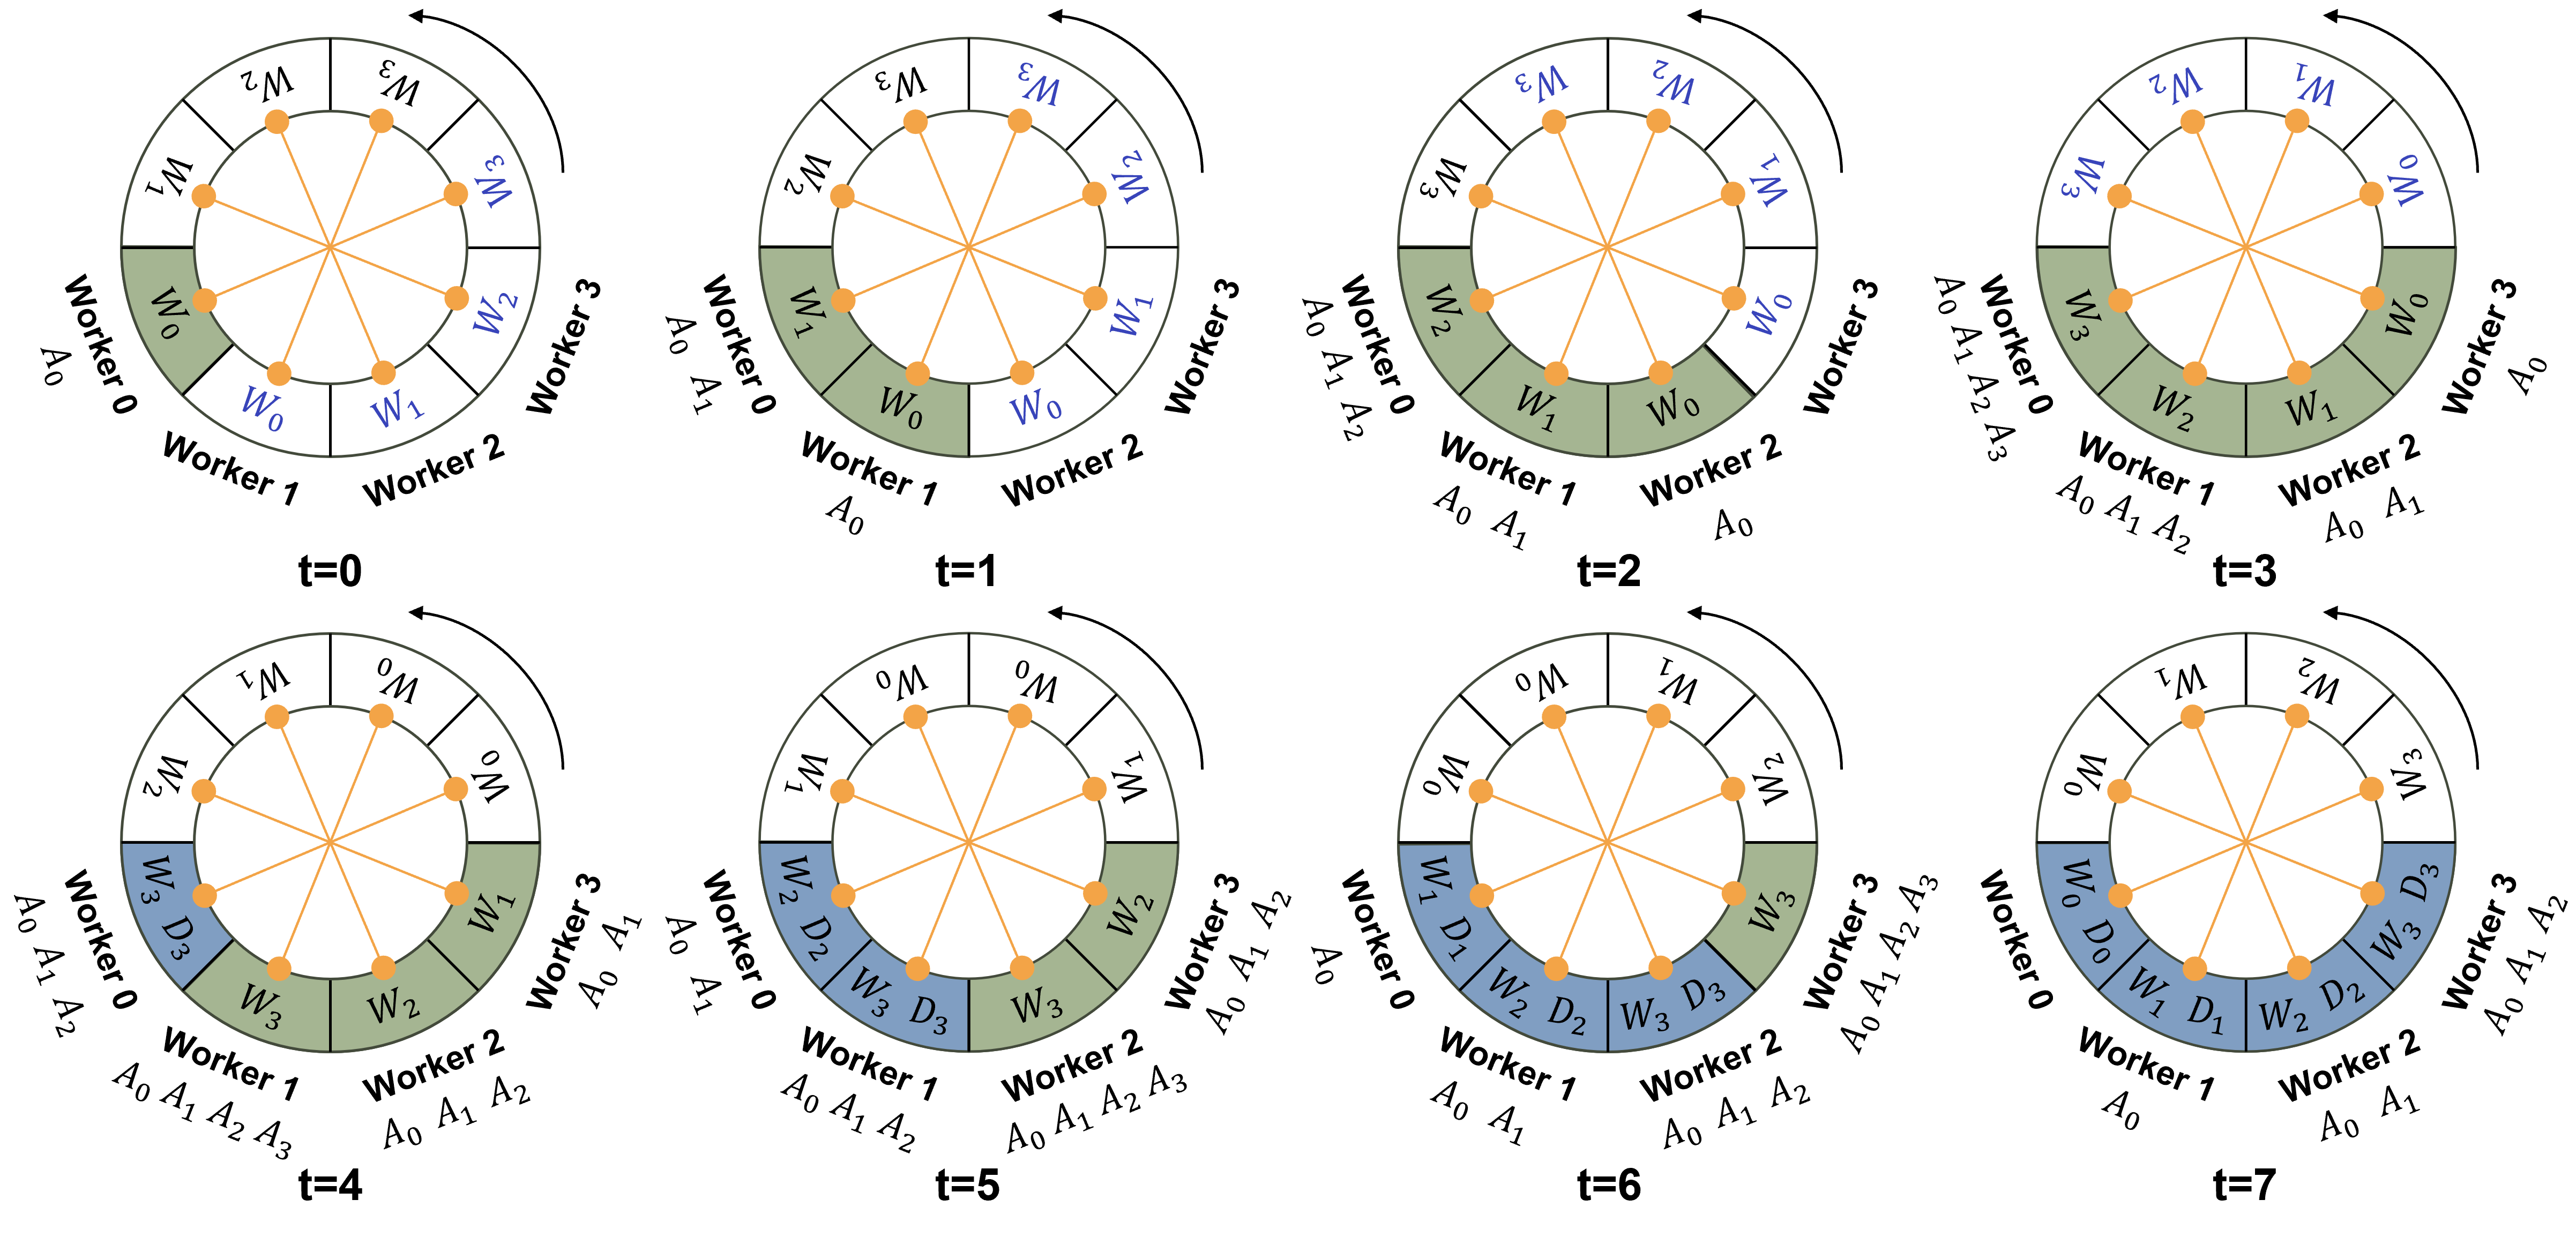
\includegraphics[scale=0.41]{figures/fig1.png}
    \caption{An example of WeiPipe-Naive strategy. The text below each worker denotes the data that it retains in memory. The text within the circle represents data circulating among workers, with the circle turning counterclockwise. At turn $t$, each worker has the data at its current position and the other side of the orange line. For instance, at $t=5$, worker 1 has $W_0$, $W_3$ and $D_3$, and receives $W_1$, $W_2$ and $D_2$ from worker 0. At $t=6$, worker 1 holds  $W_1$, $W_2$ and $D_2$. The green block indicates that the worker is currently performing the forward pass, while the blue block indicates that it is performing the backward pass.}
    \label{fig:weipipe-naive}
\end{figure*}

\subsection{Large Models and Long Context Training}
Recently, Transformer-based models \cite{vaswani2023attention, brown2020language, devlin2018bert, touvron2023llama, peebles2023scalablediffusionmodelstransformers, dosovitskiy2021vit} have become foundational across multiple fields, such as Natural Language Processing (NLP) and Computer Vision (CV). As researchers strive for better performance, the scale of these models has increased significantly in two major dimensions.

First, the size of the models themselves has grown substantially. For example, the recently released Llama-3.1 model \cite{dubey2024llama3herdmodels} boasts an impressive 405 billion parameters, necessitating at least 6480 GB of GPU memory to accommodate the model parameters. However, commonly used GPUs like the Nvidia A100 and H100 offer only 80 GB of memory each. This disparity presents a significant challenge in distributing such large models across a vast number of GPUs, with up to 16,000 Nvidia H100 units required in the case of Llama-3.1 \cite{dubey2024llama3herdmodels}.

Second, the activation size during model training has also increased due to longer sequence lengths. In NLP, long-context capabilities are crucial for tasks such as multi-round conversations\cite{openai2023gpt4}, summarization\cite{Koh2022AnES, beltagy2020longformer}, and processing large codebases\cite{li2023starcodersourceyou, rozière2024codellamaopenfoundation, chowdhery2022palmscalinglanguagemodeling}. In CV, generating high-resolution, long-duration videos\cite{Brooks_2024, peebles2023scalable} results in sequences that expand both temporally and spatially. Additionally, in scientific AI, models like AlphaFold \cite{Jumper2021Alphafold, cheng2023fastfold} must manage long sequences of amino acids. These long-context scenarios introduce new challenges in designing parallelism schemes that achieve efficient and balanced memory management.

\subsection{Parallelism Technique for Training}
To address the aforementioned challenges, various parallelization techniques have been developed. Data Parallelism is the most straightforward approach, dividing the data among devices and using an all-reduce operation at each iteration to synchronize gradients. Enhanced versions, such as FSDP \cite{zhao2023pytorchfsdpexperiencesscaling} and ZeRO-3 \cite{rajbhandari2020zeromemoryoptimizationstraining}, further optimize by splitting model weights and optimizer states.
TP \cite{shoeybi2019megatron, xu2021efficient, wang2022tesseract, li2023automatedtensormodelparallelism, cheng2023atpadaptivetensorparallelism} divides tensors into chunks along specific dimensions, allowing each device to hold only a portion of the tensor without compromising the integrity of the computation graph. This technique requires frequent collective communication to synchronize the results.
PP \cite{gems, gpipe, dapple, li2021chimera, hanayo, qi2023zerobubblepipelineparallelism} partitions the model at the layer level and splits the mini-batch into micro-batches. Traditional pipeline parallelism assigns layers across multiple devices and uses P2P communication to pass activations between devices.
Additionally, Sequence Parallelism (SP) \cite{jacobs2023Ulysses, liu2023ring, gu2024loongtrainefficienttraininglongsequence, li2022sequence, liu2024wallfacerguidingtransformermodel} splits activations along the sequence dimension. Among these parallelization strategies, Data Parallelism, particularly FSDP, is widely adopted due to its ease of use and suitability for large models. Meanwhile, Pipeline Parallelism is favored for its reliance on P2P communication, making it a viable option for devices with less robust connections. To better understand WeiPipe, we will first explore these parallelization techniques in detail.

\subsubsection{Pipeline Parallelism}

In this paper, we will primarily focus on synchronous pipelines, which maintain the convergence of the training process. One of the most well-known pipeline parallelism techniques is Gpipe \cite{gpipe}, which completes all forward propagation for all micro-batches before starting the backward propagation. Dapple \cite{dapple}, also known as 1F1B, enhances this approach by initiating backward propagation of a mini-batch immediately after its forward propagation finishes, thereby reducing peak memory requirements on certain devices. Chimera \cite{li2021chimera} further optimizes by combining multiple pipelines in different directions to reduce the bubble ratio. Hanayo builds on this by utilizing a wave-shaped pipeline to decouple Chimera from model duplication, thereby improving efficiency. Zero-Bubble Pipeline Parallelism \cite{qi2023zerobubblepipelineparallelism} introduces a technique to compute gradients for weights and activations separately, allowing for a more flexible pipeline stage arrangement. This method offers two schemes: one minimizes peak memory consumption, and the other reduces the bubble ratio. Further discussion on these approaches can be found in Section \ref{sec:analysis}. While current pipeline parallelism techniques have largely focused on reducing the bubble ratio, they face significant challenges in long-context scenarios. In these cases, the overhead from peer-to-peer (P2P) activation and gradient communication can exceed the computational load of a single pipeline stage, leading to substantial GPU idling.


\subsubsection{Fully Sharded Data Parallelism}

Fully Sharded Data Parallelism(FSDP)\cite{zhao2023pytorchfsdpexperiencesscaling} has similar functions with Zero-3\cite{rajbhandari2020zeromemoryoptimizationstraining}, sharding the data, model weights and optimizer states and distribute them on different GPUs. In FSDP, model weights and gradients are only gathered when necessary for computation and are promptly discarded after the computation is completed. This sharding and unsharding process is facilitated by all-gather and reduce-scatter operations. FSDP also incorporates asynchronous communication to enhance overlap and offers user-friendly APIs. Despite its ease of use and memory efficiency, FSDP requires a substantial amount of collective communication during both forward and backward propagation, which could be challenging in scaled scenarios.

In a word, existing techniques are not well-equipped to reduce the communication overhead in long-context scenarios, particularly in clusters with less robust network connections.

\section{WeiPipe Framework}

\subsection{WeiPipe-Naive}

\begin{figure*}[!ht]
    \centering
    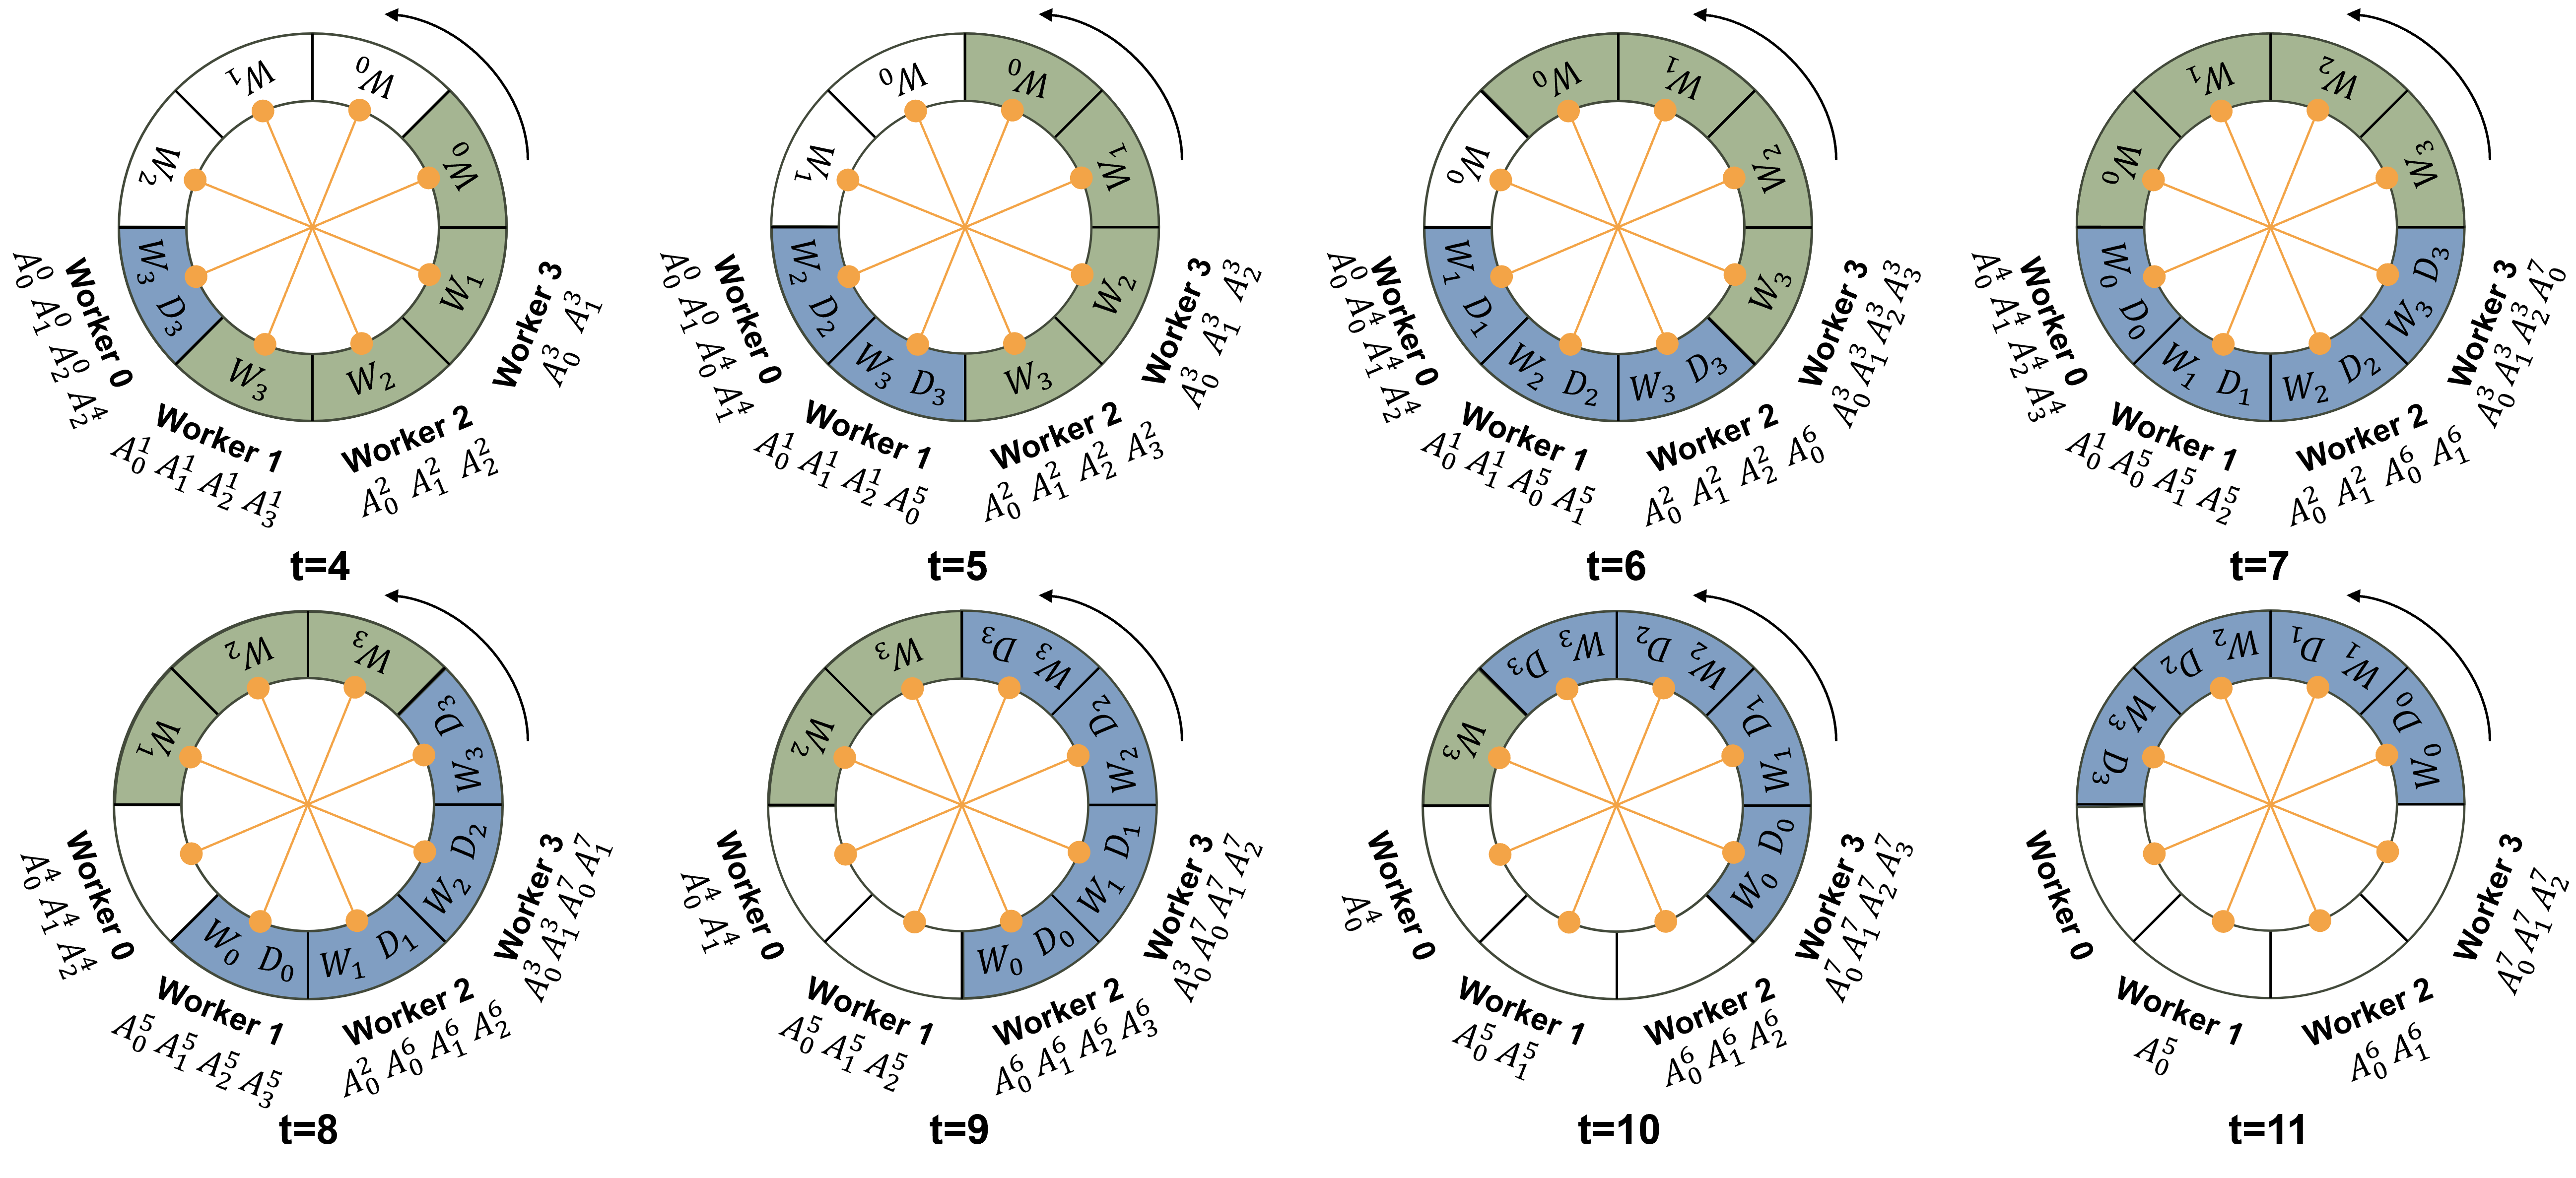
\includegraphics[scale=0.4]{figures/fig2.png}
    \caption{An example of WeiPipe-Interleave strategy. $A^i_j$ denotes the activation values of $j$th layer in $i$th micro-batch.} 
    \label{fig:weipipe-interleave}
\end{figure*}

To introduce the basic idea of WeiPipe, we focus on the commonly used ring topology PP. The initial step in pipeline training is evenly distributing the layers of the model across all workers along the ring topology, with each worker possessing part of the weights of the model. Let's just assume the number of layers $L$ is equal to the number of workers $P$. Therefore, each worker holds one layer's weight. The training procedure consists of three passes: the forward pass, the backward pass, and the update pass. During the forward pass, achieving a weight-passing pipeline is straightforward. Worker 0, holding the weights $W_0$ of the first layer, initiates the forward computation. Simultaneously, it passes $W_0$ to worker 1 and receives $W_1$ from worker $P-1$. Subsequently, worker 0 discards the $W_0$ but retains the activation values of the first layer $A_0$ on its own memory and begins computing the second layer using $W_1$. Meanwhile, worker 1 computes the first layer with a new micro-batch input. This process continues until worker 0 completes the forward pass across all layers. Figure \ref{fig:weipipe-naive} illustrates this procedure from $t=0$ to $t=3$ for $P=4$. In Figure \ref{fig:weipipe-naive}, we use a circular representation to illustrate data arrangement and transmission in WeiPipe, which is particularly helpful for understanding the complex strategies discussed in this paper. For $P=4$, the circle is divided into 8 positions, each occupied by $W$s or $D$s. Each worker holds data at its current position and at the diagonal position (indicated by the orange line across the circle). Initially, worker 0 through worker 3 each hold $W_0$ to $W_3$ respectively (as shown by the black text in the circle). The circle rotates counterclockwise, with each turn denoted as $t+1$. After each rotation, workers update the data they hold, reflecting the transition of data between workers. Each worker processes the forward pass for its corresponding layer (indicated by the green block in the circle), and accumulates activation values from $A_0$ to $A_3$ in their own memory, as shown below each worker. 

The backward pass becomes more complex because weights are required in reverse order. To maintain the weight-pipelining, we fill the opposite side of the circle with $W_3$ to $W_0$, as illustrated in the blue text in Figure \ref{fig:weipipe-naive} from $t=0$ to $t=3$. After Worker 0 completes the forward pass, the circle continues to rotate counterclockwise. Worker 0 then receives $W_3$ to $W_0$ one by one and executes the backward computation from layer 3 to layer 0 (blue blocks in Figure \ref{fig:weipipe-naive}). In WeiPipe-Naive, workers with lower numbers finish earlier than those with higher numbers. This means that while a smaller-numbered worker starts to perform the backward computation, a larger-numbered worker might still be engaged in the forward computation. Thus, weights for both forward and backward need to be transferred simultaneously. To facilitate this, each worker holds weights for both forward and backward passes. Figure \ref{fig:weipipe-naive} from $t=4$ to $t=8$ presents the backward pass of worker 0 and worker 0 can initiate another cycle for inputs of a new micro-batch after $t=8$. 

During the update pass, each worker utilizes the weight gradients ($D$s) to update the weights. However, since weights cycle among workers and each worker just generates a piece of $D$s for their micro-batch, updating the weights of a layer requires gathering all corresponding $D$s. In DP, the all-reduce primitive is used to collect $D$s. WeiPipe aims to use only P2P communications, so $D$s also circulate through the ring topology after it is generated. Taking worker 0 in Figure \ref{fig:weipipe-naive} as an example, at time $t=4$, worker 0 performs the backward pass for layer 3 with $W_3$ and generates $D_3$. Then, $D_3$ travels together with $W_3$ around the circle. Each worker that processes layer 3 propagation will average, sum, or normalize the newly generated $D_3$ with the existing $D_3$ and keep the communication volume unchanged. This circular process repeats until all micro-batches are processed, at which point each worker updates the $W$s and $D$s it holds using the specified optimizer. Since each worker updates one layer of weights, it also stores the corresponding layer of optimization state, which does not need to be transmitted between workers.

% It should be noticed that the communication of $D$s continues during a worker's forward pass, as shown in Figure \ref{fig:weipipe-naive} from $t=8$ to $t=12$. 

\subsection{WeiPipe-Interleave for Lower Bubble Ratio}  

\begin{figure*}[!ht]
    \centering
    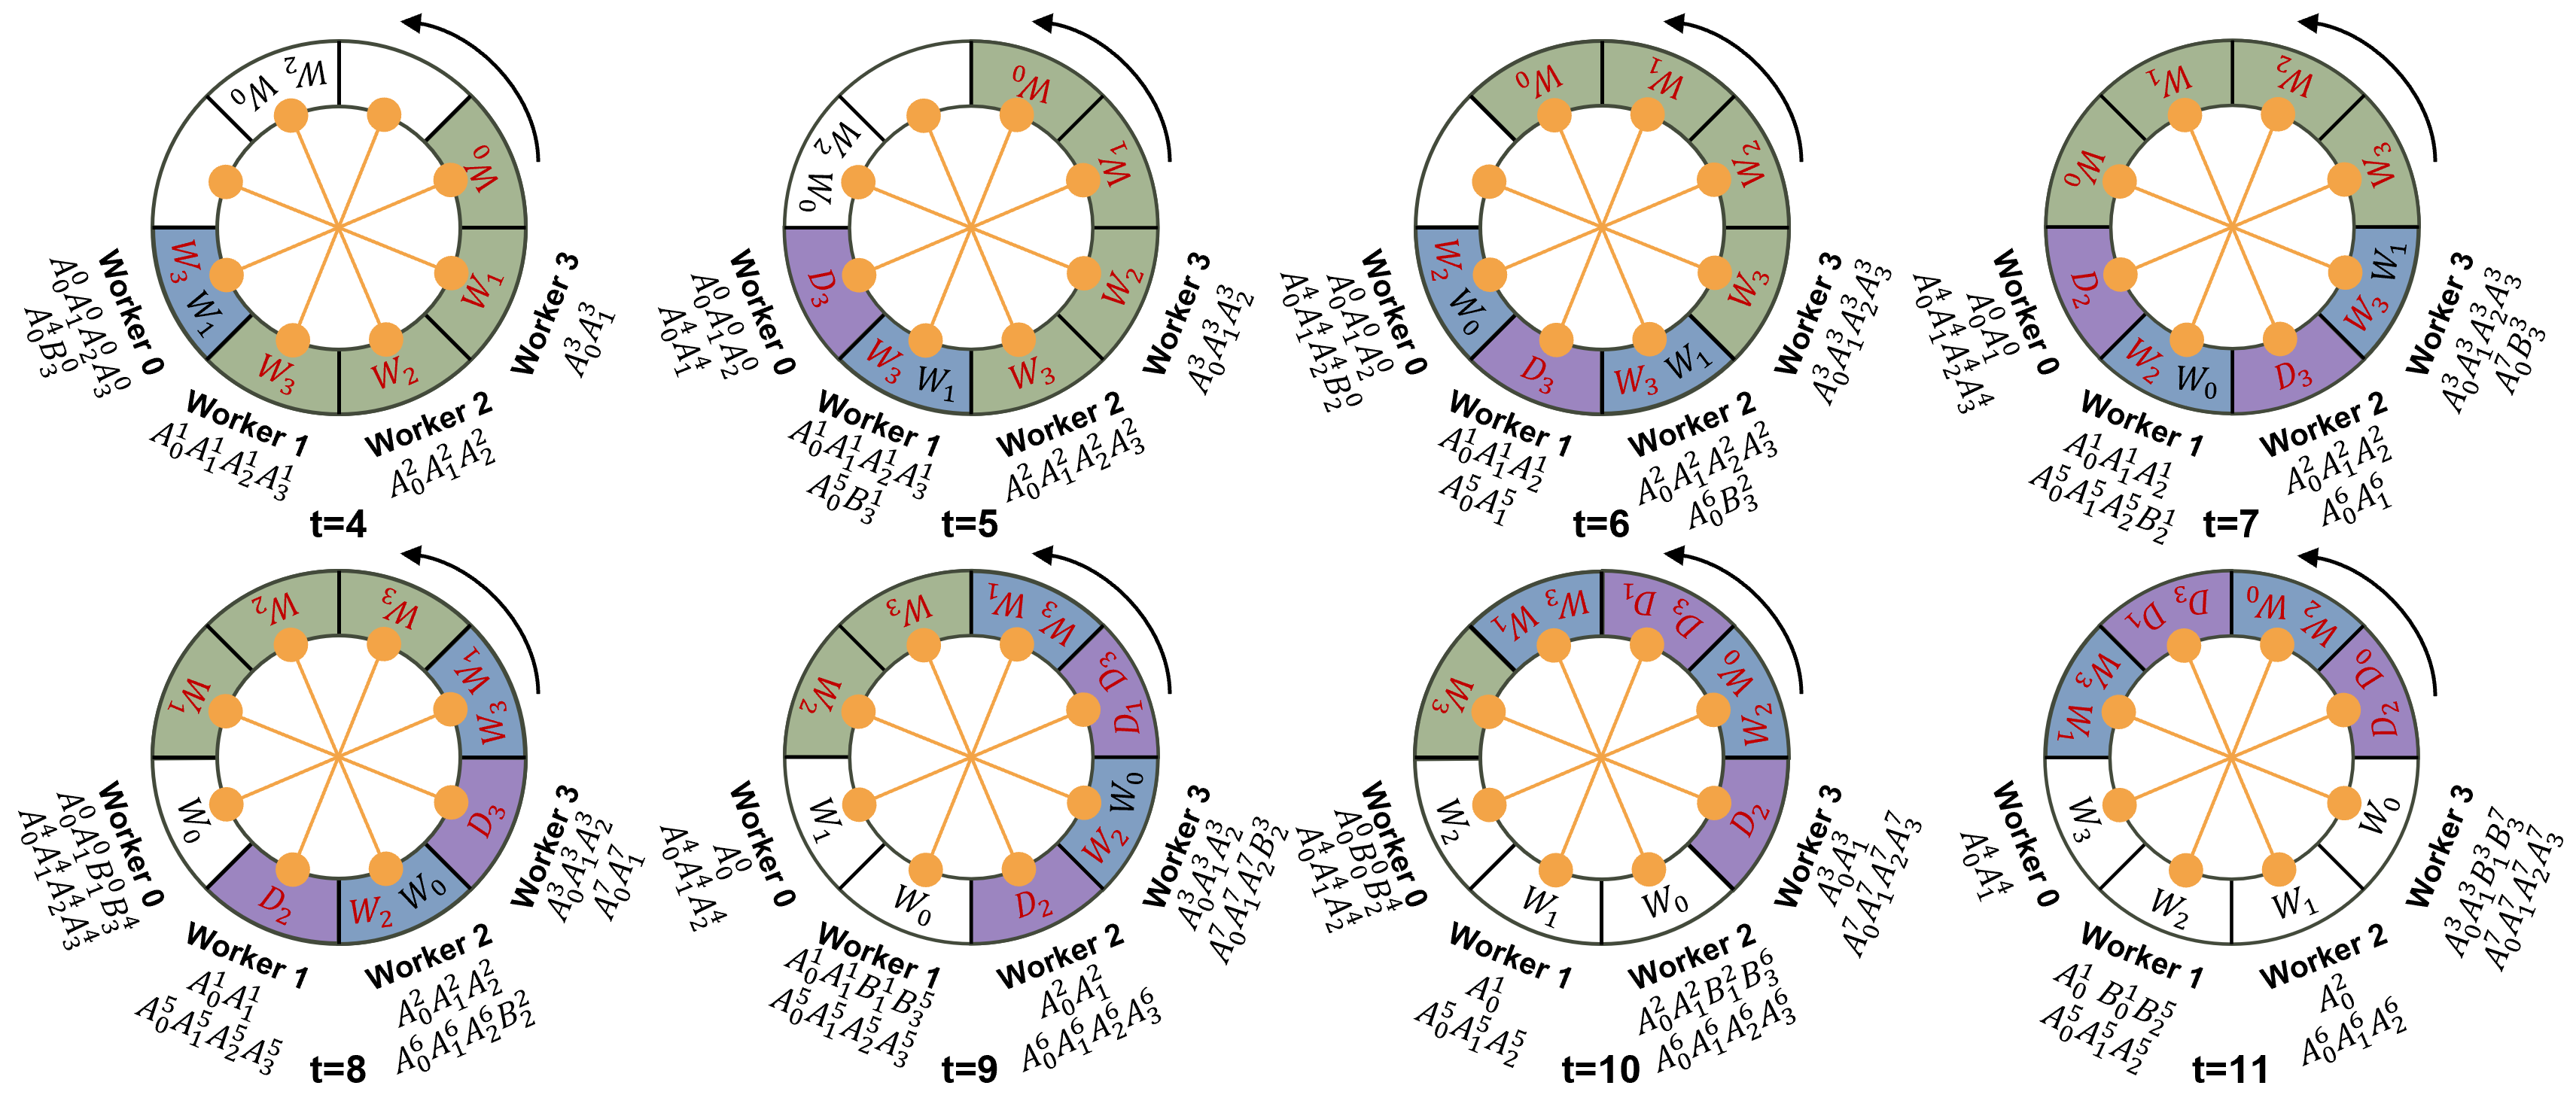
\includegraphics[scale=0.63]{figures/fig3.png}
    \caption{An example of WeiPipe-Zero-Bubble 1. Green block for the forward pass, blue block for the B pass, and purple block for the W pass. $B^i_j$ denotes the gradients of activation values of $j$th layer in $i$th micro-batch. The intermediate gradient values between layers are ignored in this Figure.} 
    \label{fig:weipipe-zero-1}
\end{figure*}

There are major flaws of WeiPipe-Naive. Firstly, the memory utilization among workers fluctuates rather than being balanced. Secondly, there are two weight-flow circulating simultaneously, but only one is used for the current computation. The redundant transmission of weights inflates transmission costs. Most crucially, the computational time for the backward pass of a layer is approximately twice that of the forward pass. When one worker executes the backward pass, it significantly increases the pipeline bubble for other workers currently engaged in the forward pass. To address these issues, we interleave the forward and backward pass and get the WeiPipe-Interleave strategy. 

The idea is to utilize the weights at the diagonal positions of the circle for another micro-batch forward or backward computation. The initial forward process is the same as WeiPipe-Naive. Figure \ref{fig:weipipe-interleave} illustrates the interleaving forward and backward computations from $t=4$ to $t=11$. At $t=4$, worker 0 begins to perform the backward pass. In the meantime, it utilized the $W_0$ to perform the forward pass of a new micro-batch's input. Therefore, at this position, worker 0 will execute one backward and one forward before the circle makes another turn. During this time, other workers can only perform one forward operation and wait for worker 0’s computation to finish. In the subsequent turn, workers 0 to 3 also enter the forward-backward interleave stage when the computation workloads are balanced between works. 

There is no pipeline bubble during the forward-backward interleave stage no matter how different the workloads of backward and forward are. Each worker can also decide their own executing order for the forward and backward passes based on their data transmission situation. Moreover, idle memory during the forward and backward pass is utilized for storing activation values generated by new micro-batches, as shown in Figure \ref{fig:weipipe-naive}, which results in a balanced storage utilization across different workers and at different times. WeiPipe-Interleave further reduces communication overhead during the interleaving stage. For the LLama structure that has $12H^2$ parameters in one layer. During the forward-backward interleave stage, each worker will receive two layers of weights and one layer of $D$ in each turn. The communication volume is $36H^2$, which is half of the $72H^2$ in naive WeiPipe. 

\subsection{WeiPipe-Zero-Bubble} 
\label{sec:zero_bubble}

\begin{figure*}[!ht]
    \centering
    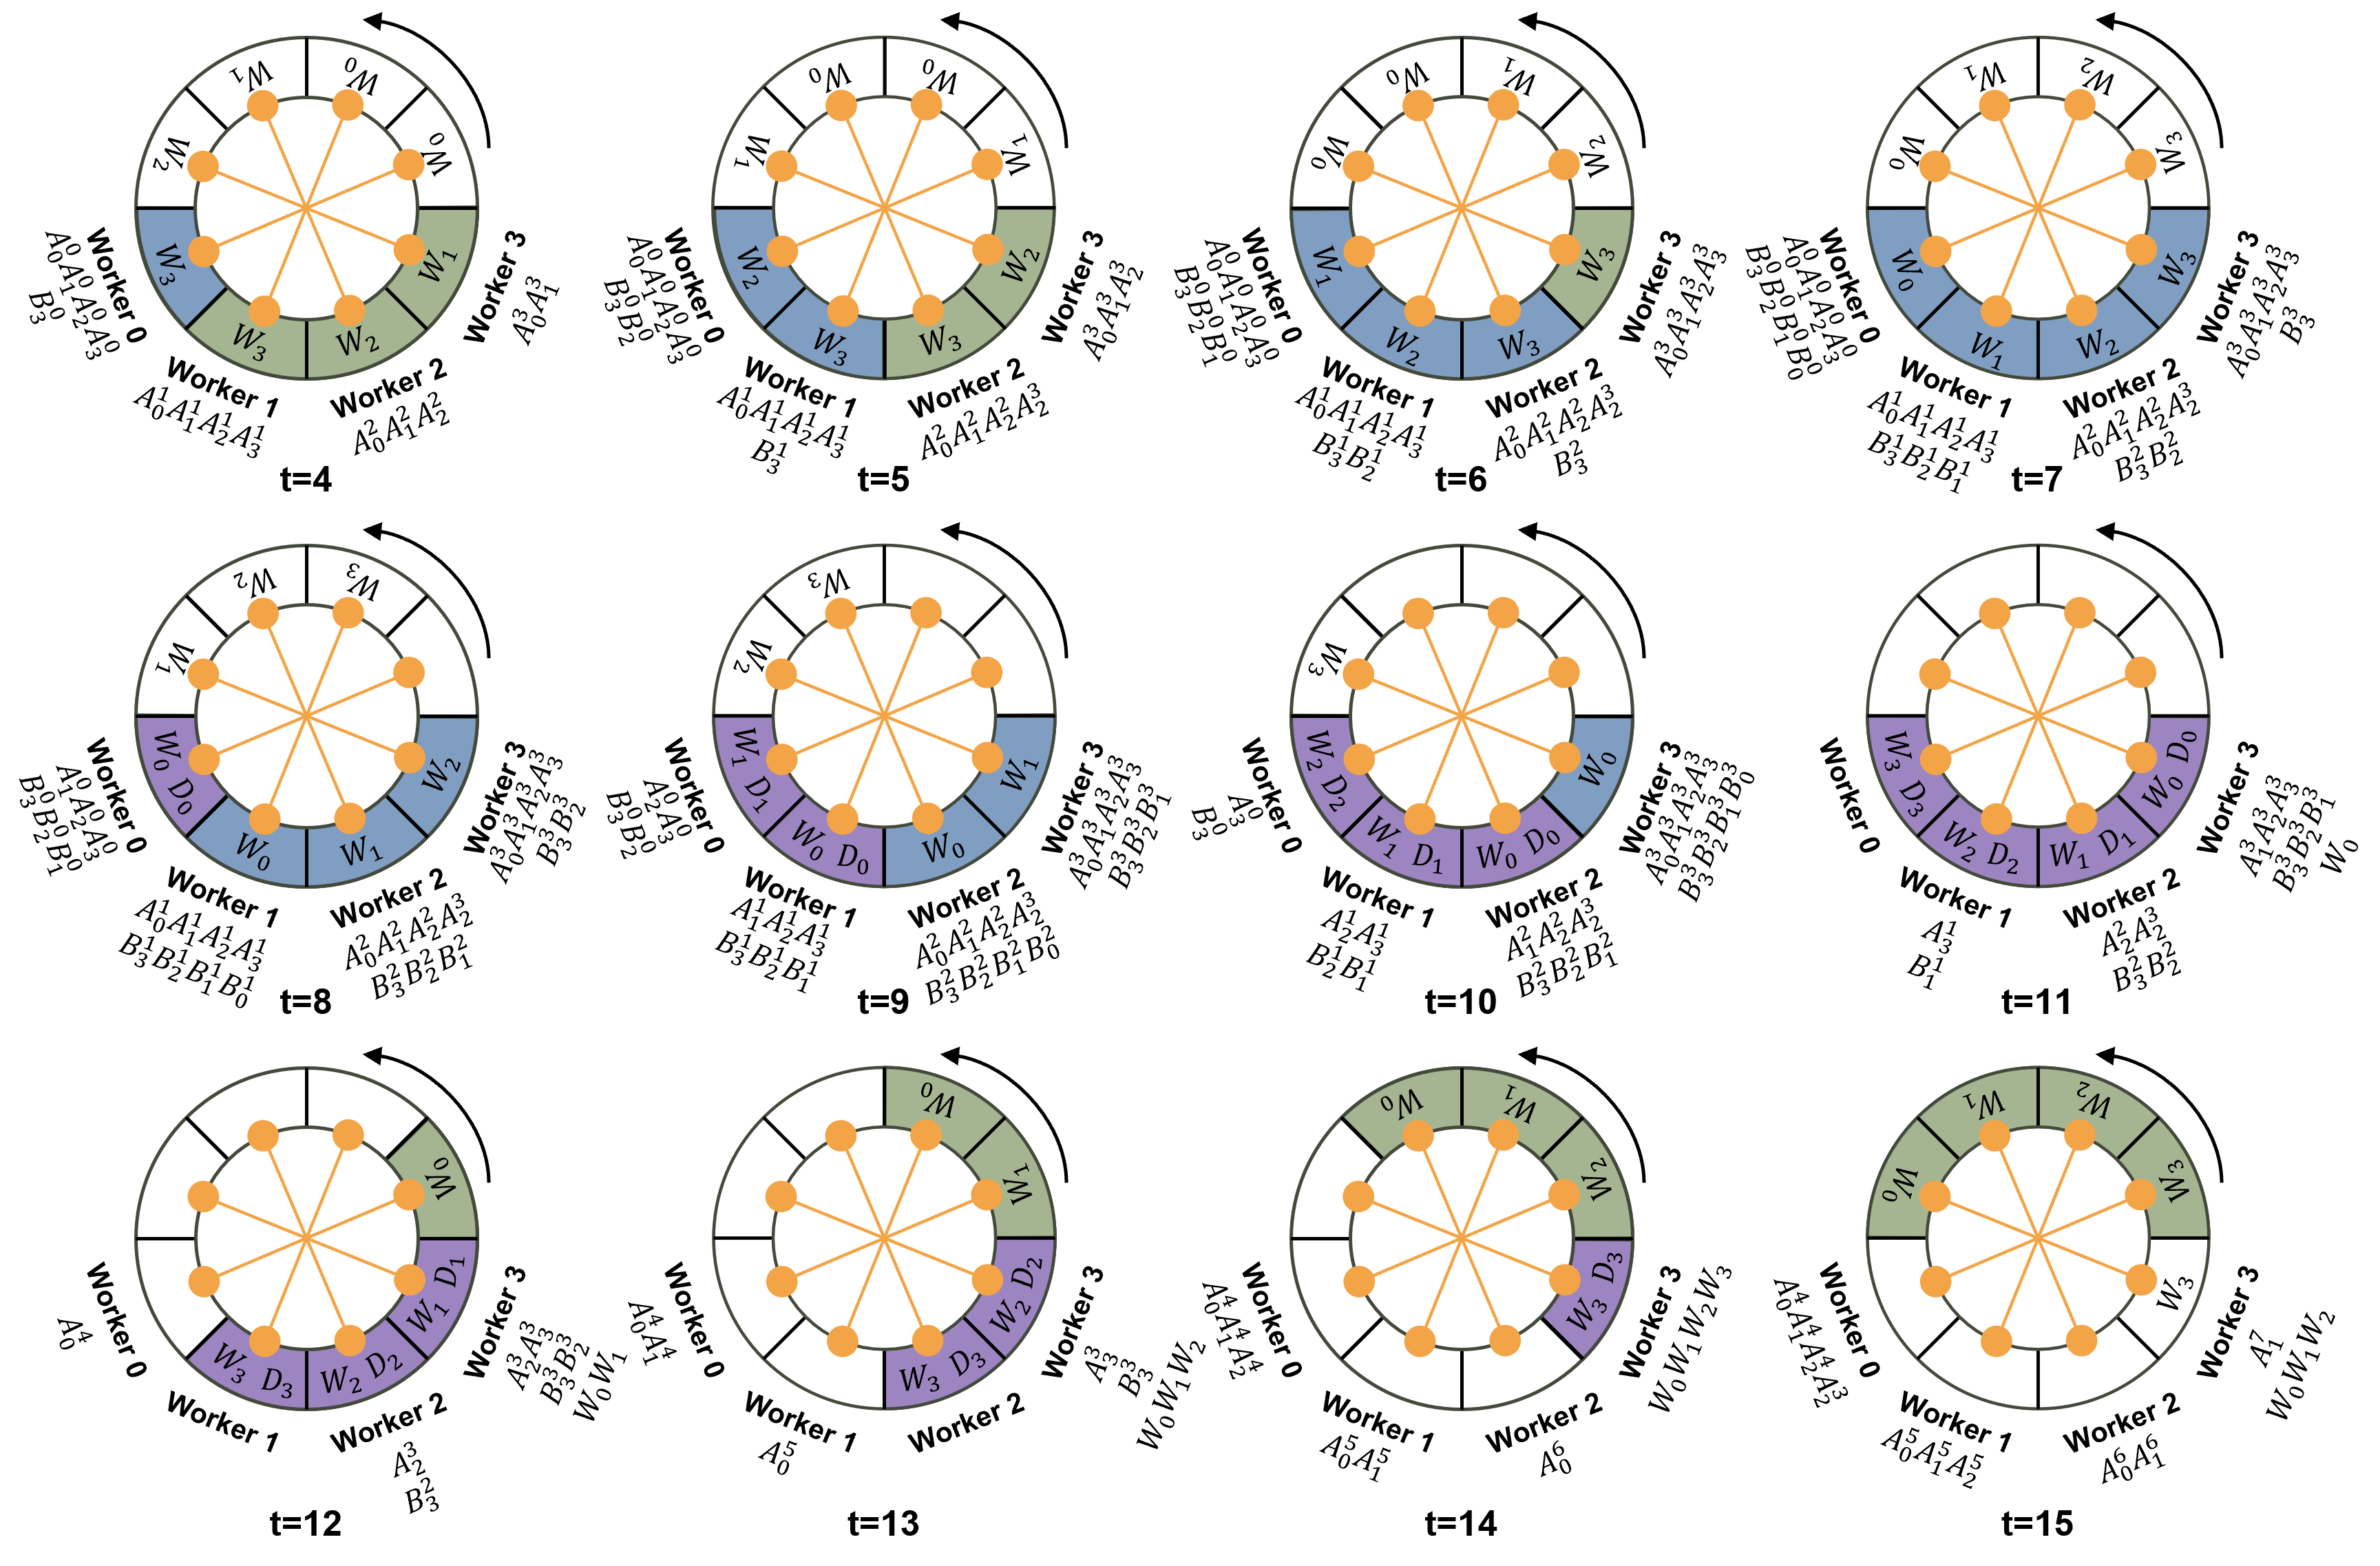
\includegraphics[scale=0.61]{figures/fig4.png}
    \caption{An example of WeiPipe-Zero-Bubble 2. The worker 3 stages the updated weights at the end of each round and delivers these weights one by one to the worker 0 for the next round. This arrangement will not exceed the peak memory of worker 3.} 
    \label{fig:weipipe-zero-2}
\end{figure*}

To further explore the potential of WeiPipe, we present a design that combines WeiPipe with the Zero-Bubble pipeline. Zero-Bubble strategies are state-of-the-art PP that split the backward computation into B pass and W pass to achieve almost zero-bubble. In Zero-Bubble, the B pass computes gradients for inputs and activations, and the W pass computes gradients for the weights. The B pass is performed in a backward manner while the W pass can be delayed to fill the blanks in the pipeline. Inspired by this, We introduce WeiPipe-Zero-Bubble 1, which slightly reduces the bubble ratio compared to WeiPipe-Interleave with relatively low storage and communication overhead, and WeiPipe-Zero-Bubble 2, which achieves a nearly zero bubble configuration. 

Figure \ref{fig:weipipe-zero-1} shows the procedure of WeiPipe-Zero-Bubble 1 from $t=4$. Blue blocks represent B passes, while purple blocks denote W passes. At $t=4$, worker 0 conducts two tasks: forward of layer 0 on a new micro-batch (micro-batch 4) with $W_0$, generating $A_0^4$; the B pass of layer 3 with $W_3$ on the old micro-batch (micro-batch 0), producing the activation gradient $B_3^0$. Worker 0 still retains part of the $A_3^0$ after $t=4$ for the future W pass on $W_3$. Different from WeiPipe-Interleave, $W_1$ for the backward pass is placed together with the $W_3$ in the circle. The red text in Figure \ref{fig:weipipe-zero-1} indicates the data used by the worker at the current turn. At $t=5$, worker 0 performs the W pass, consuming $A_3^0$ and $B_3^0$ to generate $D_3$ on the circle, which will be sent to the worker 1. Simultaneously, worker 0 also conducts micro-batch 4's forward with $W_1$. This process continues with alternating "one-forward-one-B" and "one-forward-one-W" until the forward pass of micro-batch 4 is completed. Then, at $t=8$, worker 0 performs two B passes--one for micro-batch 0 with $W_1$ and one for micro-batch 4 with $W_3$. From $t=8$ to $t=11$, worker 0 alternates between two B passes and two W passes until $t=12$ when all passes for micro-batch 0 are completed, and the forward pass for a new micro-batch (micro-batch 8) begins. 

Figure \ref{fig:weipipe-zero-1} illustrates the data arrangement on the ring. $W_0$ to $W_3$ for the forward pass are consistent with the previous strategy. Weights for the B pass and gradients generated by the W pass are both placed in pairs. Generally, for a network with $L$ layers, $W_{L-1}$ and $W_{\frac{L}{2} -1}$ are placed together, $W_{L-2}$ and $W_{\frac{L}{2} -2}$ are placed together, and so forth. The same pairing applies to $D$s. This arrangement ensures that each worker performs 2-chunk operations while transmitting 3 chunks of data to the next worker within one turn.

% Figure \ref{fig:weipipe-zero-1} also depicts the accumulated memory of each worker. The peak memory of a worker, excluding temporary storage for $W$s and $D$s, is about $\frac{3}{2}M_A$, where $M_A$ denotes for.

Compared to WeiPipe-Zero-Bubble 1, WeiPipe-Zero-Bubble 2 offers a more simple procedure with the same $W$s and $D$s arrangement as WeiPipe-Interleave, as shown in Figure \ref{fig:weipipe-zero-2}. In WeiPipe-Zero-Bubble 2, the forward, B, \& W passes for all layers are executed sequentially within a worker. Notably, the W pass progresses from layer 0 to layer 3, matching the forward's order. During the B pass, old versions of weights can be discarded to reduce transmission, as indicated by the blanks from $t=8$ to $t=11$. The last worker, worker 3, aggregates all $D$s and updates the weights. In the case in Figure \ref{fig:weipipe-zero-2}, at $t=11$, worker 3 holds the aggregated $D_0$ updates $W_0$ with specified optimizer. Worker 3 then sends the updated $W_0$, which initiates a new forward pass at $t=12$. This seamless handover allows for frequent weight updates with fewer micro-batches and achieves almost zero bubble ratio. Typically, WeiPipe-Zero-Bubble 2 incurs higher communication and storage costs. Usually, it performs 1-chunk operation while transmitting 2 chunks of data to the next worker.

% or distributes the $D$s to other workers with corresponding optimizer state in next round of circling

\section{Theoretical Analysis}
\label{sec:analysis}

\begin{figure*}[!htb]
    \centering
    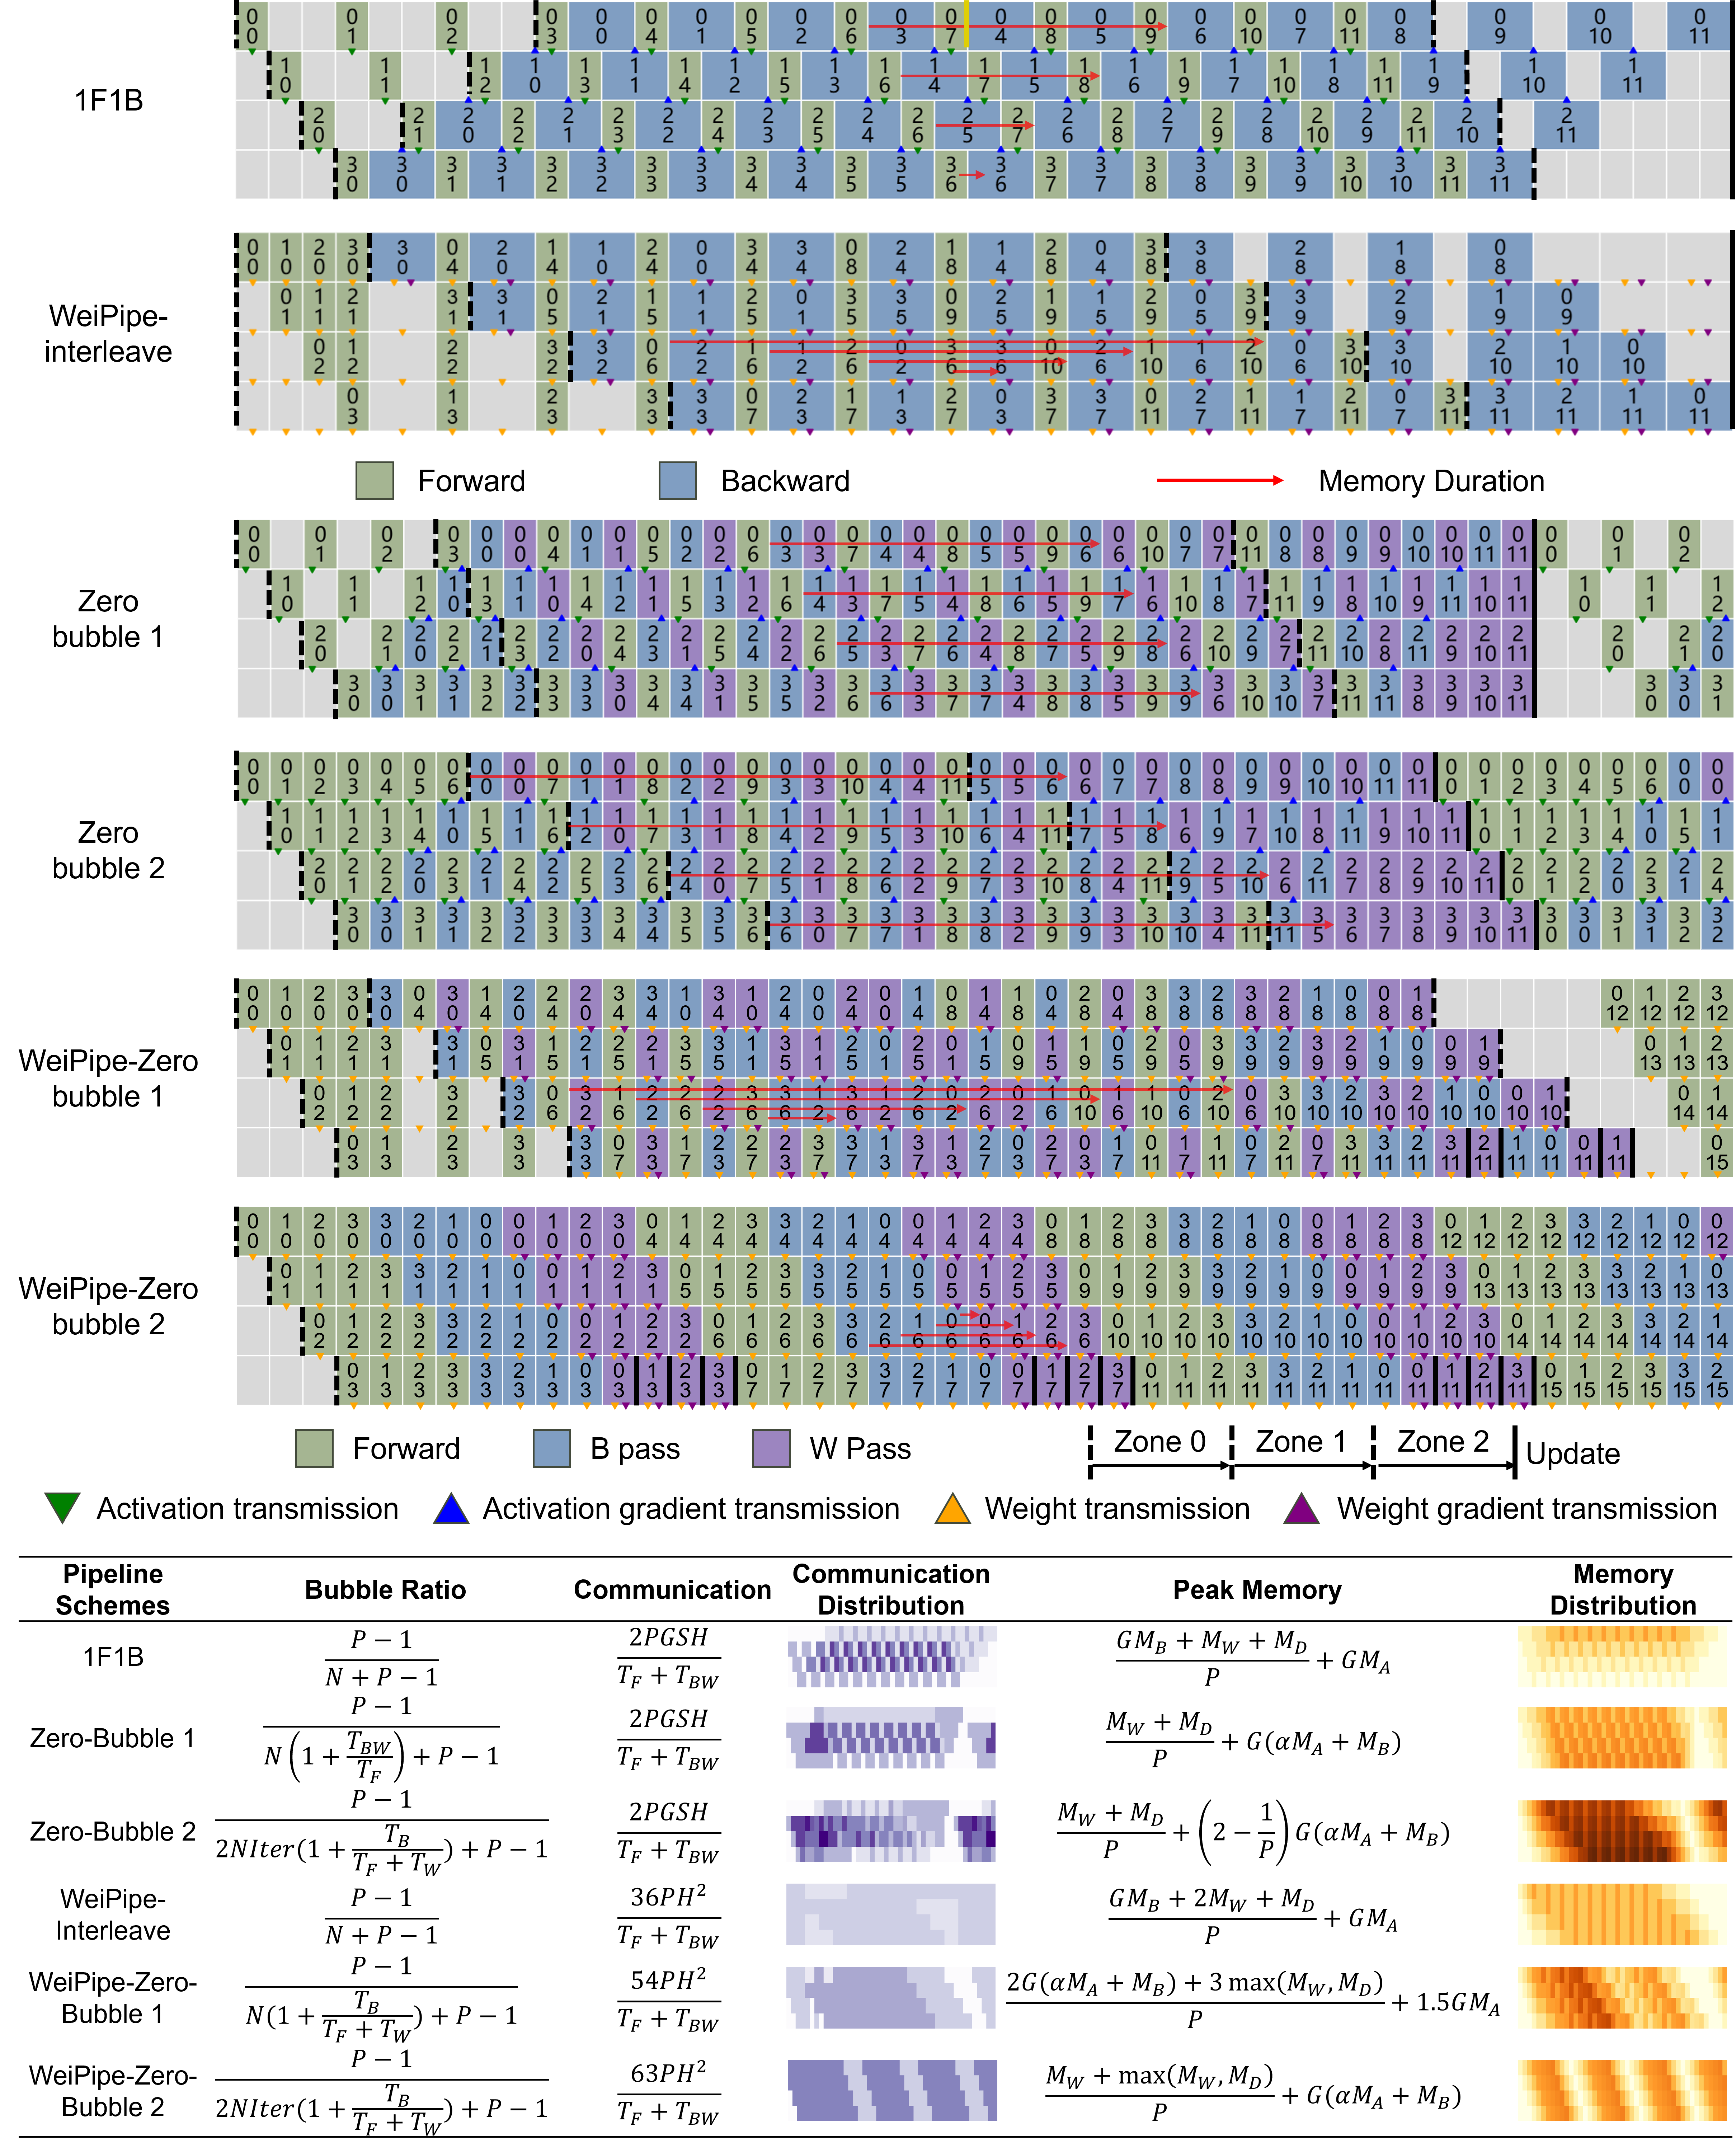
\includegraphics[scale=0.43]{figures/fig5.png}
    \caption{The comparison of WeiPipe with other pipeline strategies. In the pipelining graph, the upper number in a block represents the layer index and the bottom number is the micro-batch index. The distribution graph in the equation table shows the theoretical bandwidth and memory usage of these strategies along devices and times. The specific value is calculated based on Llama-structure with $H=4096$, $S=4096$, $N=12$, $G=32$, and 32 heads Transformer. Memory distribution is estimated with $\alpha=0.6$ without recomputation and flash attention. The practical distribution could be distinct depending on implementation.}
    \label{fig:weipipe-comparision}
\end{figure*}

Figure \ref{fig:weipipe-comparision} compares WeiPipe with other pipeline parallelism. WeiPipe-Interleave has the same bubble ratio as 1F1B. Both zero-bubble strategies reduce the bubble ratio by multiplying a factor greater than 1 to $N$ in the bubble ratio equation. Zero-Bubble 2 and WeiPipe-Zero-Bubble 2 have almost no bubbles along the iteration. 

% Specifically, the factor $1+\frac{T_{BW}}{T_F}$ in Zero-Bubble 1 with lower bubble ratio is larger than $1+\frac{T_B}{T_F + T_W}$ in WeiPipe-Zero-Bubble 1. 

Communication efficiency is assessed by dividing the total number of received data by the computation time (Bandwidth usage). Different zones of a pipeline strategy have different communication densities. Figure \ref{fig:weipipe-comparision} presents the equation of theoretical bandwidth usage of Zone 1, where passes are fully alternated (Zone 0 for WeiPipe-Zero-Bubble 2). For activation-passing strategies, the equation is derived from middle workers transmitting both $A$s and $B$s (So, there is a "2" in the equation). Communication for activation-passing strategies increases linearly with micro-batch size $G$ and sequence length $S$. In contrast, WeiPipe’s communication is dictated by the amount of weights, independent of $G$ and $S$. In this paper, LLama-style Transformers are selected as standard models for analysis, where the number of weights per layer is $12H^2$. WeiPipe-Interleave requires transmitting two chunks of $W$ and one chunk of $D$, resulting in a communication volume of $36H^2$ at each turn with a time duration of $\frac{T_F + T_W}{P}$, where $T_F$ and $T_F$ is the time for a complete forward and backward respectively. Consequently, WeiPipe-Interleave outperforms other strategies in terms of communication when $\frac{GS}{18H} > 1$. When $\frac{GS}{27H} > 1$, WeiPipe-Zero-Bubble 1 has a communication advantage over Zero-Bubble strategies.


% Peak memory usage is similar to 1F1B, though WeiPipe-Interleave stores additional weights for the simultaneous forward and backward passes of different layers.

Memory consumption is significantly impacted by the specific implementations. Here, we provide a rough estimation of $M_A$, $M_B$, $M_W$, and $M_D$ based solely on the counts of these values, while ignoring factors such as communication buffers, embedding layers, and mixed-precision training. For 1F1B and WeiPipe-Interleave, the dominating part is the storage for activations, measured as $GM_A$. WeiPipe-Interleave has similar memory consumption with 1F1B but with more balanced utilization. In strategies that separate the B pass and W pass, one stage of the B pass ($\frac{1}{P}$ of a complete B pass) will consume part of the activation values $M_A/P$ stored by the forward pass and generate gradients $M_B/P$. We assume that $\alpha M_A/P$ activations storage is left after one stage of B pass in a worker. For Zero-Bubble strategies, we assess the peak storage required by the last worker. Zero-Bubble 1 and WeiPipe-Zero-Bubble 2 both need to store $G(\alpha M_A+M_B)$ data. The Zero-Bubble 2 nearly doubles this requirement. However, WeiPipe-Zero-Bubble 1 can achieve peak memory consumption of approximately $1.5GM_A$, which is less than other zero-bubbles strategies when $\frac{M_B}{M_A} > 1.5-\alpha $. It should be noted that calculating the peak memory for Zero-Bubble 1 could be tricky. With smaller $\alpha$ and specific memory management strategies in GPU, worker 0 may have the largest memory consumption. 

% \subsection{Comparison with other pipeline parallel strategies} 

% \subsection{Comparison with other data parallel strategies} 

% \subsection{The resilience} 

% \begin{figure*}[!ht]
%     \centering
%     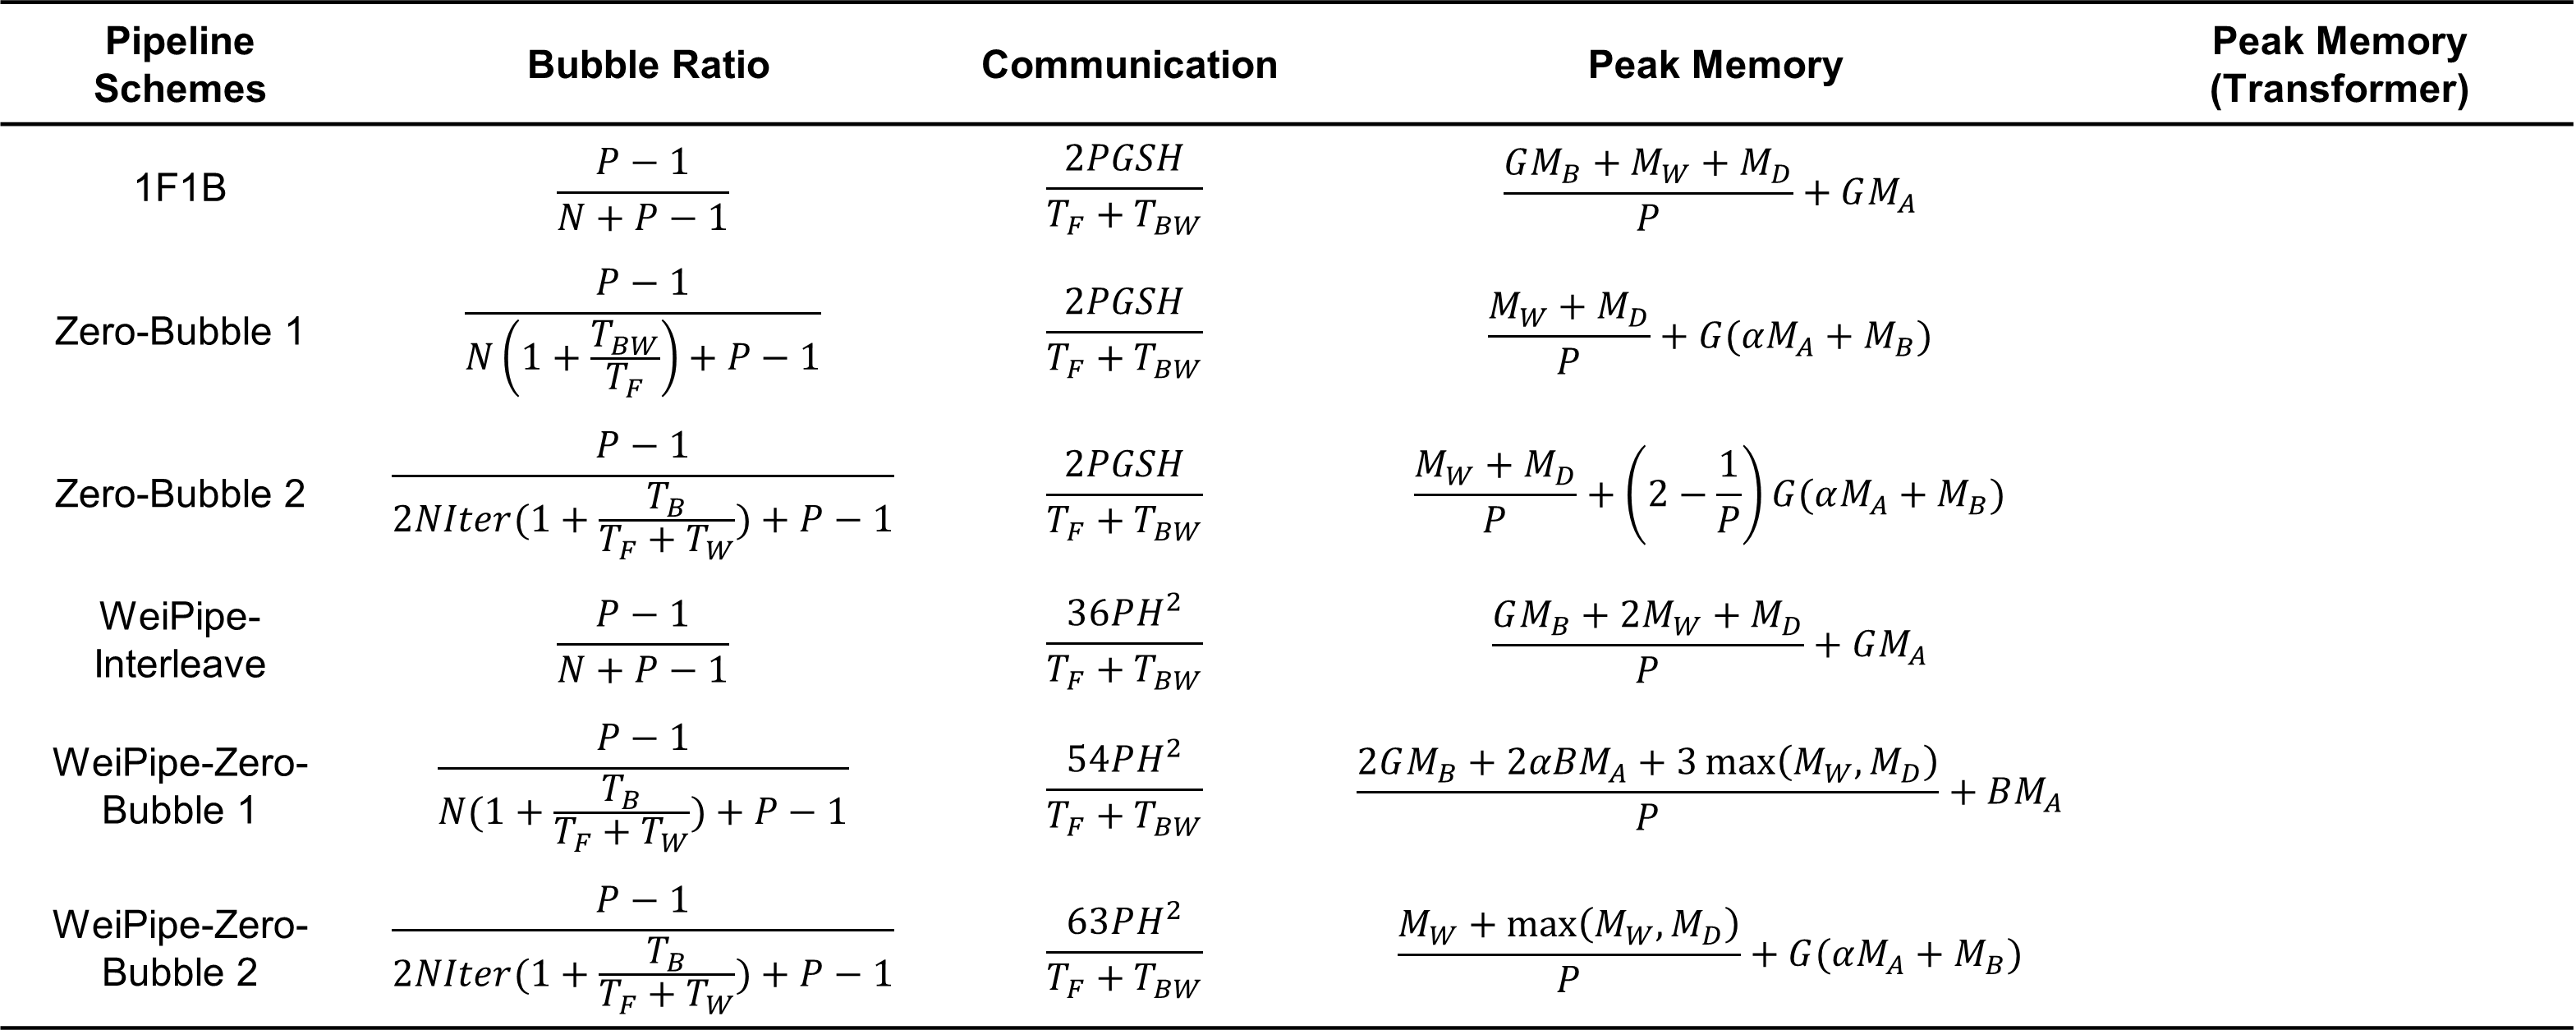
\includegraphics[scale=0.65]{figures/table1.png}
%     \caption{The comparison of WeiPipe with other pipeline strategies}
%     \label{fig:weipipe-comparision_table}
% \end{figure*}


% 1F1B
% latency hidden

\section{Implementation} 

Current distributed training frameworks offer various activation-passing pipeline strategies, but few accommodate high-level modifications to achieve weight pipelining. Thus, we have implemented WeiPipe-Interleave from scratch in PyTorch\cite{pytorch}. The implementation is tailored for training LLMs, but our approach is not limited to Transformers. Due to the need for intricate and fined-grained control, we present WeiPipe-Zero-Bubble to demonstrate the potential of a weight-passing pipeline and to facilitate a deeper discussion, while leaving the implementation for future exploration. The following details are considered for implementation:

% \subsection{Mixed Precision} 
\textbf{Mixed Precision.} Unlike other pipeline research that primarily focuses on full precision implementation, our implementable incorporates widely adopted mixed precision training to further reduce memory consumption and communication. Specifically, $A$, $W$, and $D$ are in fp16 precision, while $B$ is in bf16. The optimizer state is in fp32, distributed among workers, and does not need to be transmitted between workers in WeiPipe-Interleave. 

% \subsection{Overlap by prefetching}

% \begin{figure*}[!ht]
%     \centering
%     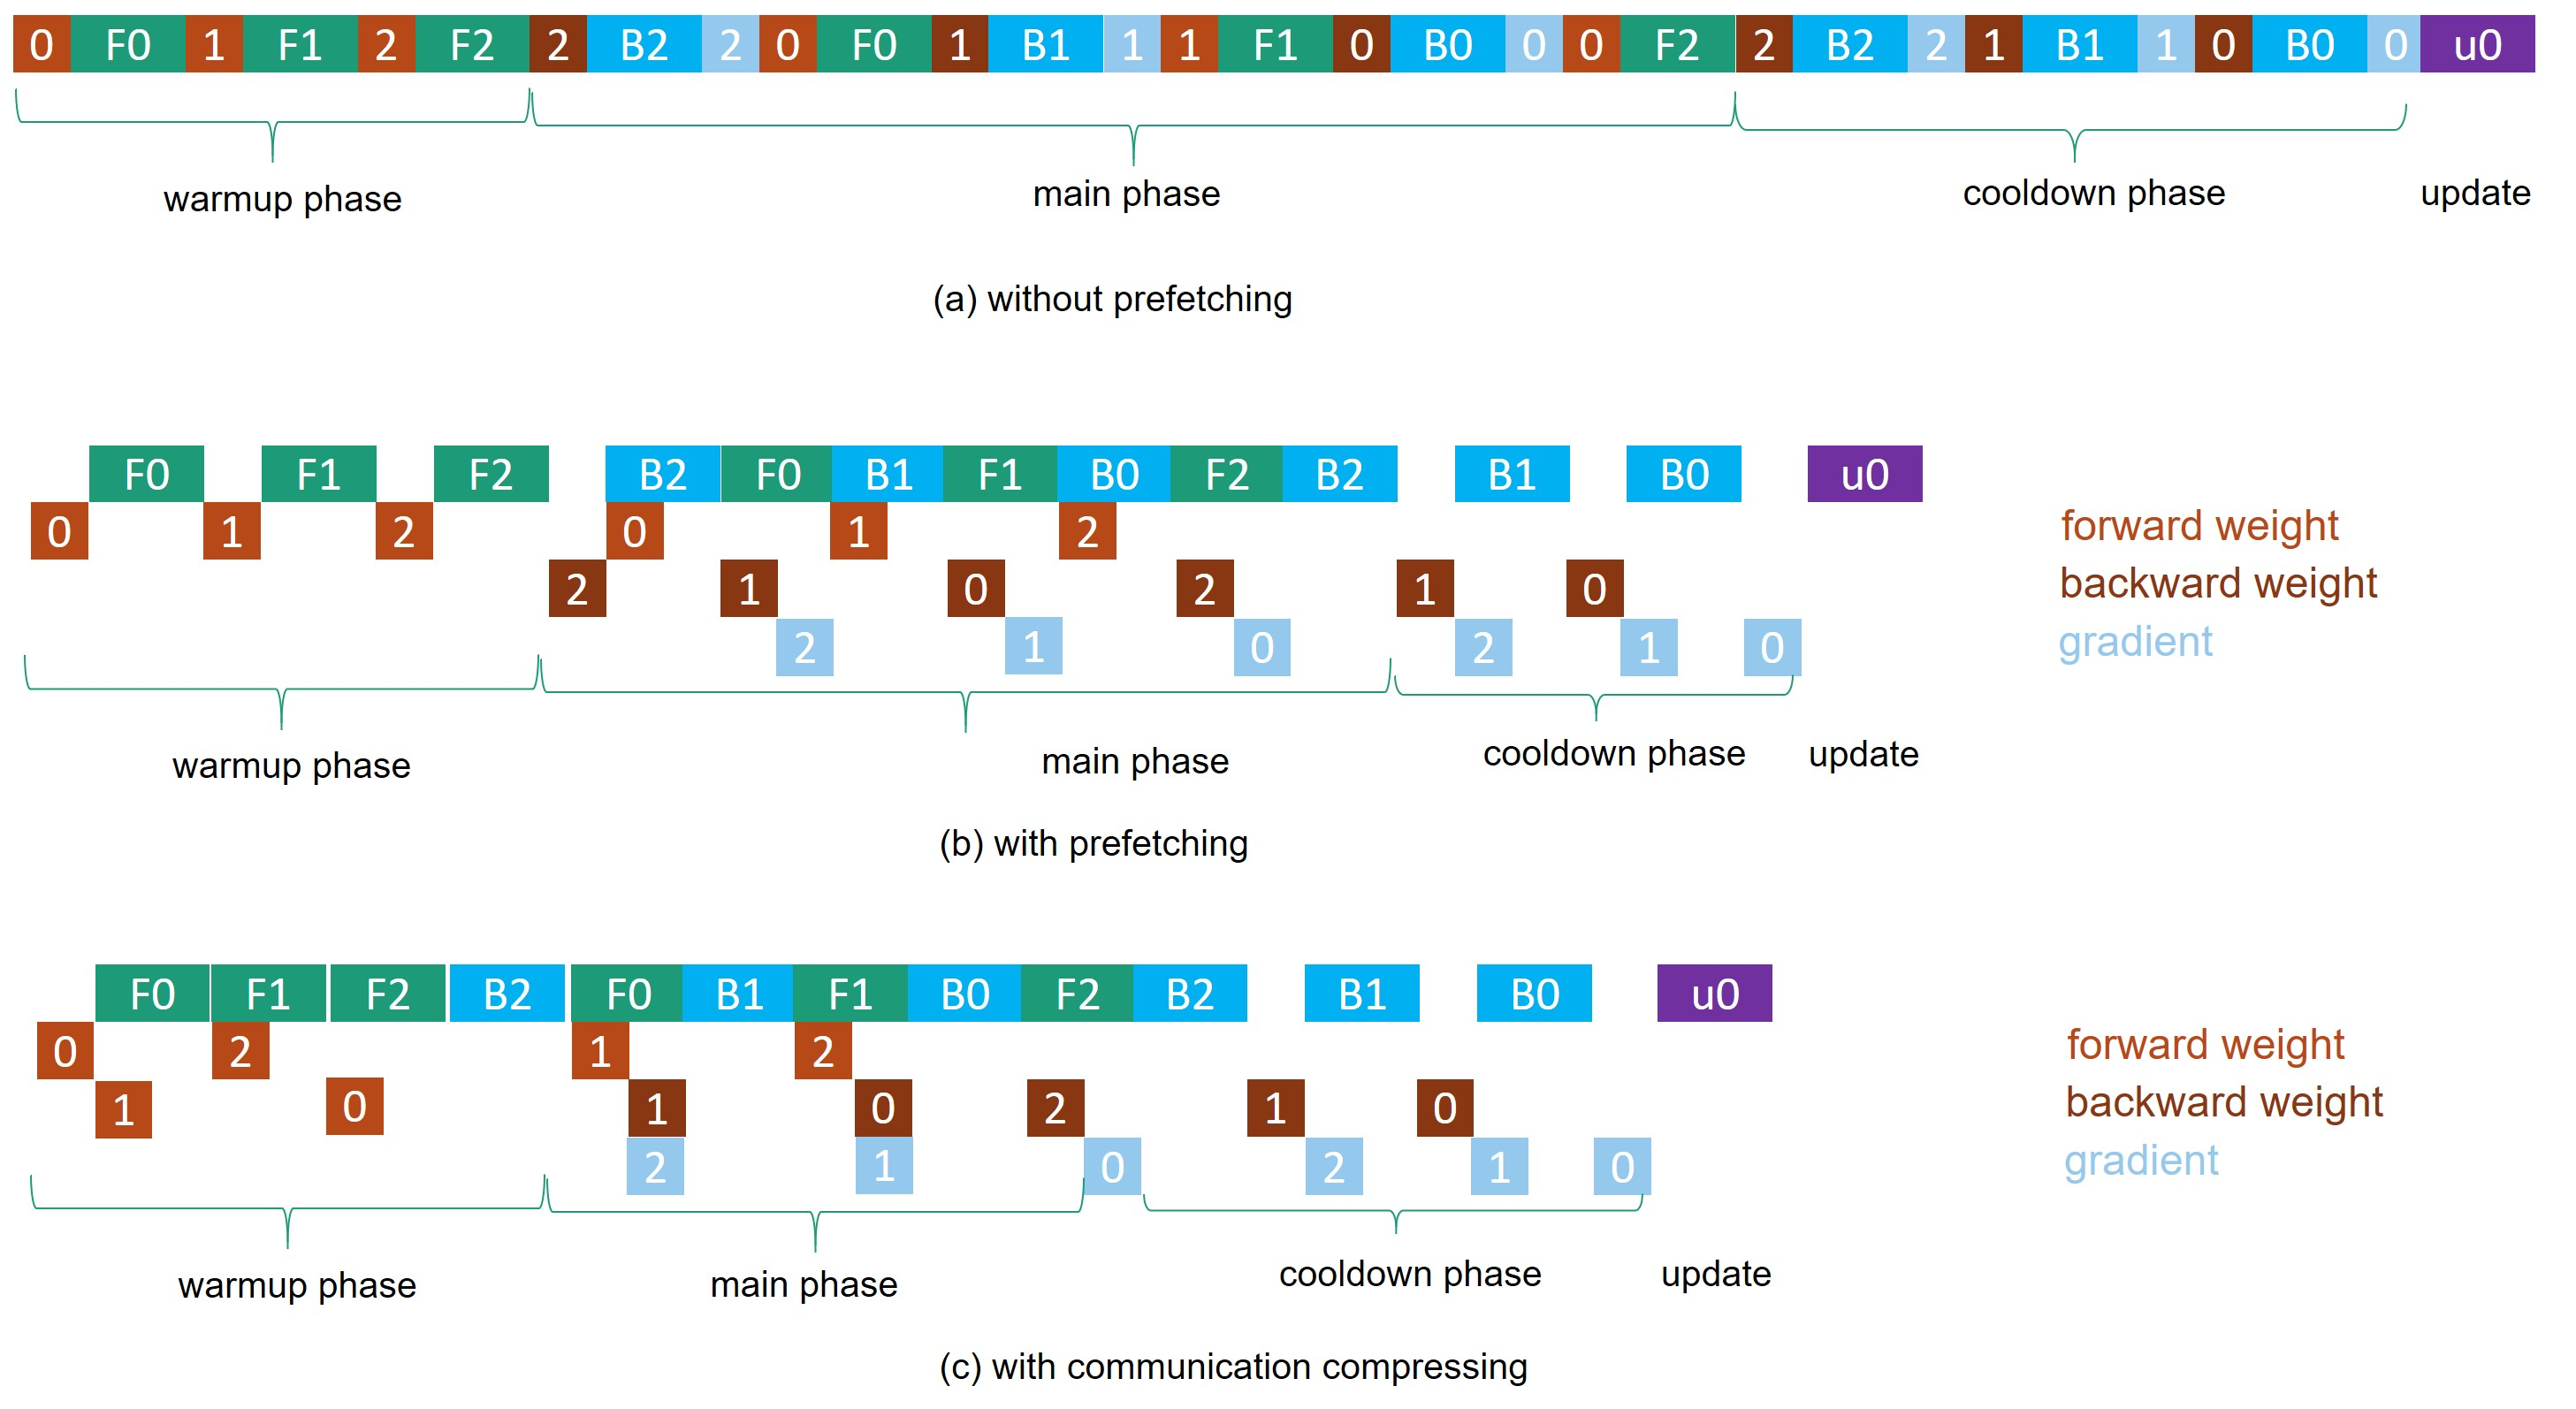
\includegraphics[scale=0.7]{figures/overlap.jpg}
%     \caption{Overlap by prefetching}
%     \label{fig:overlap}
% \end{figure*}

\textbf{Communication overlap.} WeiPipe meticulously adjusts the arrangement of computation and weight-passing to balance the communication and computation workload. To ensure WeiPipe's high-performance potential is realized, fine-grained communication hiding optimizations are implemented. During forward-backward interleaving, $W$s and $D$s are prefetched using asynchronous communication, which is realized by utilizing the batch\_isend\_irecv function provided by PyTorch NCCL backend.

\textbf{Recomputation and Flash Attention.} Recomputation (gradient checkpointing/rematerialization) is a strategy that saves storage by abandoning part of activation values during the forward pass. Instead, these values are recomputed during the backward pass, thus significantly reducing memory consumption with some redundant computation. Similarly, Flash Attention\cite{dao2022flashattention} is a widely used technique to optimize memory access and save memory in attention modules. By employing these techniques, we can increase micro-batch size and enhance the strengths of WeiPipe. We also implement these optimizations across other strategies for a fair comparison.


\begin{table*}[!ht]
\centering
% Please add the following required packages to your document preamble:
% \usepackage{multirow}
\begin{tabular}{ccc|ccccc|ccccc}
\hline
\multicolumn{3}{c|}{Model Config}                & \multicolumn{5}{c|}{Troughput(Tokens/second)}         & \multicolumn{5}{c}{Memory(GB)}          \\
S                      & N                   & G & 1F1B    & ZB1    & ZB2    & FSDP   & WeiPipe          & 1F1B  & ZB1   & ZB2   & FSDP  & WeiPipe \\ \hline
\multirow{4}{*}{4096}  & \multirow{2}{*}{16} & 4 & 46,217  & 48,259 & 50,027 & 56,014 & \textbf{135,405} & 2.41  & 6.26  & 10.73 & 3.48  & 3.85    \\
                       &                     & 8 & 49,799  & 51,200 & 52,937 & 91,022 & \textbf{145,960} & 4.52  & 12.22 & 21.16 & 6.73  & 7.28    \\
                       & \multirow{2}{*}{32} & 4 & 50,374  & 52,513 & 53,368 & 65,080 & \textbf{112,605} & 2.41  & 6.26  & 10.73 & 3.48  & 3.88    \\
                       &                     & 8 & 53,586  & 55,515 & 56,158 & 89,104 & \textbf{118,832} & 4.52  & 12.22 & 21.16 & 6.73  & 7.34    \\ \hline
\multirow{4}{*}{8192}  & \multirow{2}{*}{16} & 4 & 49,536  & 51,160 & 52,054 & 74,220 & \textbf{123,188} & 4.57  & 12.26 & 21.2  & 6.73  & 7.28    \\
                       &                     & 8 & 51,441  & 52,788 & 53,961 & 82,125 & \textbf{124,593} & 8.79  & 24.18 & 42.06 & 13.21 & 14.14   \\
                       & \multirow{2}{*}{32} & 4 & 53,784  & 55,003 & 55,563 & 77,557 & \textbf{99,979}  & 4.57  & 12.26 & 21.2  & 6.73  & 7.34    \\
                       &                     & 8 & 55,563  & 56,606 & 57,312 & 83,247 & \textbf{101,685} & 8.79  & 24.18 & 42.06 & 8.79  & 14.27   \\ \hline
\multirow{4}{*}{16384} & \multirow{2}{*}{16} & 4 & 50,783  & 52,013 & 53,109 & 58,988 & \textbf{92,239}  & 8.98  & 24.37 & 42.24 & 13.21 & 14.14   \\
                       &                     & 8 & 51,471  & 52,650 & OOM    & 60,015 & \textbf{92,729}  & 17.42 & 48.2  & OOM   & 26.18 & 27.86   \\
                       & \multirow{2}{*}{32} & 4 & 54,957  & 55,657 & 56,351 & 59,255 & \textbf{73,636}  & 8.98  & 24.37 & 42.24 & 13.21 & 14.27   \\
                       &                     & 8 & 55,498  & 56,478 & OOM    & 60,145 & \textbf{73,937}  & 17.42 & 48.2  & OOM   & 26.18 & 28.11   \\ \hline
\end{tabular}
\caption{Throughput and peak memory of training the LLama-style model on 8 GPUs with NVLink connections.}
\label{tab:perform_nvlink}
\end{table*}

\section{Evaluation}

% Memory
% Speed
% Communication Volume v.s. PP
% MFU



\begin{table}[!ht]
\centering
% Please add the following required packages to your document preamble:
% \usepackage{multirow}
\begin{tabular}{ccc|ccccc}
\hline
\multicolumn{3}{c|}{}                         & \multicolumn{5}{c}{Troughput(Tokens/second)}                          \\
S                   & N                   & G & 1F1B            & ZB1    & ZB2    & FSDP            & WeiPipe         \\ \hline
\multirow{4}{*}{s1} & \multirow{2}{*}{16} & 4 & \textbf{11,877} & 9,802  & 10,373 & 8,540           & 10,234          \\
                    &                     & 8 & 11,781          & 9,755  & 10,412 & 15,319          & \textbf{19,734} \\
                    & \multirow{2}{*}{32} & 4 & \textbf{12,783} & 10,047 & 10,406 & 8,439           & 9,898           \\
                    &                     & 8 & 12,824          & 10,144 & 10,501 & 14,755          & \textbf{19,787} \\ \hline
\multirow{4}{*}{s2} & \multirow{2}{*}{16} & 4 & 11,875          & 9,760  & 10,487 & 14,328          & \textbf{19,361} \\
                    &                     & 8 & 11,761          & 9,999  & 20,975 & 21,755          & \textbf{25,655} \\
                    & \multirow{2}{*}{32} & 4 & 12,891          & 10,048 & 10,411 & 14,236          & \textbf{18,091} \\
                    &                     & 8 & 12,727          & 10,034 & 20,822 & 21,751          & \textbf{23,044} \\ \hline
\multirow{4}{*}{s3} & \multirow{2}{*}{16} & 4 & 11,704          & 9,950  & OOM    & 18,503          & \textbf{21,576} \\
                    &                     & 8 & 11,556          & OOM    & OOM    & \textbf{23,542} & 21,994          \\
                    & \multirow{2}{*}{32} & 4 & 12,610          & 9,978  & OOM    & 18,338          & \textbf{19,518} \\
                    &                     & 8 & 12,316          & OOM    & OOM    & \textbf{23,330} & 19,914          \\ \hline
\end{tabular}
\caption{Throughput of training LLama-style models on 16 GPUs from 2 clusters with PCIe connections within cluster. s1, s2, and s3 represents 4096, 8192, 16384 respectively.}
\label{tab:perform_pcie}
\end{table}

\subsection{Experimental Setup}

We evaluate our implementation on models based on the open-source LLama-2 structure\cite{touvron2023llama2openfoundation} (also GPT-style models). In our experiments, we fix the head number as 32 and the hidden dimension size $H$ as 1024. We change the layer number $L$, token length $S$, micro-batch size $G$, and the number of micro-batches $N$ in an iteration to get models with various scales. We compared the WeiPipe-Interleave against widely-used 1F1B, state-of-the-art Zero-Bubble 1 \& 2, and FSDP under different communication infrastructures in terms of throughput, memory consumption, and scalability. The 1F1B and Zero-Bubble strategies are implemented through Megatron-LM, while FSDP is achieved by the Zero-3 optimization in DeepSpeed. All strategies are applied with the same model configuration, micro-batch size, mixed-precision settings, recomputation, flash-attention, and hardware environment. 

% \begin{itemize}
%     \item Can WeiPipe outperform other strategies in models with long token lengths or on low-bandwidth infrastructures?
%     \item Can WeiPipe maintain balanced and efficient memory utilization to support large micro-batch sizes?
%     \item Can WeiPipe achieve both weak and strong scalability as the conventional pipeline parallelism? Specifically, how does WeiPipe’s scalability compare to FSDP, which also transmits $W$s and $D$s but relies on collective communications and layer synchronization?
% \end{itemize}

We choose Colossal Cloud with A800 GPUs as an experimental hardware environment. The A800 has 80GB HBM and 312 TFlops fp16/bf16 tensor cores. However, compared to the A100 GPUs, the A800 limits NVLink bandwidth from approximately 600GB/s to about 400GB/s. To evaluate the communication effectiveness of WeiPipe, we conducted experiments using two different communication infrastructures. The first setup involves 8 A800 GPUs in one cluster with NVLink\cite{nvlink} connections. The second setup features 32 A800 GPUs across 4 clusters but with PCIe connections within each cluster. Clusters are connected by InfiniBand (IB). We utilized the NCCL as the underlying communication library. The NCCL chooses ring all-reduce in FSDP within a cluster by default. Therefore, overall, we keep a ring topology for all of the parallel strategies in experiments.

\subsection{Throughput and Memory Consumption}

For NVLink environment, the performance and peak memory consumption of WeiPipe and other strategies are shown in Table \ref{tab:perform_nvlink}. In this experiment, the sequence length ranges from 4096 to 16384, covering scenarios with long context. Each sequence length has 4 different configurations for the number and size of micro-batch. Among all 12 model configurations, WeiPipe demonstrates higher performance compared to other strategies. Specifically, when $S=16384$, WeiPipe achieves 33.2\%, 30.9\%, and 22.9\% improvement of throughput compared to the 1F1B, Zero-Bubble 1, and FSDP respectively. The Zero-Bubble 2 parallelism encounters out-of-memory (OOM) under this configuration. 

Table \ref{tab:perform_pcie} presents the throughput in PCIe and IB environment with 16 A800 GPUs from 2 clusters. Compared to NVLink, this environment dramatically increases the communication pressure of large-context training. From the Table \ref{tab:perform_pcie} we can see that WeiPipe-Interleave achieves 82\% improvement of throughput compared to other PP approaches, when $S=16384$. FSDP and WeiPipe-Interleave have fluctuating throughput performance with each outperforming the other at times when $S=16384$, but at $S=8192$, WeiPipe can outperform FSDP by 17.9\%.

% The memory consumption basically aligns with theoretical analysis. 1F1B has the smallest memory usage among all pipeline strategies. Because recomputation and Flash Attention provide more significant memory savings for 1F1B. Because Zero-Bubble should retain the partial activations after the B pass. These activations are only eliminated after the corresponding W pass. The memory consumption for the WeiPipe strategy is a little more than 1F1B and FSDP, due to the additional buffer for communication. In WeiPipe-Interleave, we allocated 3 buffers to receive $W$s and $D$s and 3 buffers to send in each worker. In 1F1B, they don't allocate a whole buffer for all activations. Therefore, there is still optimization space for our approach. 


% \begin{table}[!ht]
%     \centering
%     \begin{tabular}{cccccccc}
%     \hline
%        Model  &  L & Heads  & $H$ & $S$ & $P$ &  $G$ & $G$  \\
%        1.5B & 22 & 24 & 2304 & 1024 & 8 & 6 & 24/32/64 \\
%        1.5B & 22 & 24 & 2304 & 1024 & 8 & 6 & 24/32/64 \\
%        1.5B & 22 & 24 & 2304 & 1024 & 8 & 6 & 24/32/64 \\
%        1.5B & 22 & 24 & 2304 & 1024 & 8 & 6 & 24/32/64 \\
%     \hline
%     \end{tabular} 
%     \caption{Models and settings used in this paper}
%     \label{tab:setting}
% \end{table}

% compared methods:
% \begin{itemize}
%     \item WeiPipe: Weight pipeline with interleaved schedule 
%     \item 1F1B and 1F1B-I
%     \item ZB-1p and ZB-2p: zero bubble schedules are introduced by
    
% \end{itemize}
% The implementation of 1F1B, 1F1B-I and ZB are based on the open-source Megatron-LM project. 



% In the following section, we focus on addressing the following questions:
% \begin{itemize}
%     \item What is WeiPipe's memory consumption like in practice? 
%     \item How does WeiPipe perform in diverse network scenarios?
%     \item How does WeiPipe perform in weak scaling settings, where the computing resources and tasks increase simultaneously?
%     \item How does Hanayo perform in strong scaling settings, where the goal is to use more computing resources to accelerate a fixed?
% \end{itemize}

% peak memory consumption Figure

% \subsection{comparison to data parallel}

% \subsection{Adaptability Across Diverse Network Environments}


% To assess the performance and the adaptability of different pipeline strategies across various communication infrastructures, we set up three environments:

% \begin{itemize}
%     \item A cloud server with 16 NVIDIA A100 GPUs, each with 80GB of memory, connected through \textbf{Nvlink}.
%     \item A cloud server with 16 NVIDIA A100 GPUs, each with 80GB of memory, connected through \textbf{PCIe}.
% \end{itemize}

Table \ref{tab:perform_nvlink} also presents the peak memory usage of each strategy. 1F1B has the smallest memory usage among all pipeline strategies.  Among all pipeline strategies, 1F1B exhibits the smallest memory consumption. Recomputation and Flash Attention notably reduce memory usage for 1F1B and the earlier workers in the Zero-Bubble strategy. However, for the last worker in Zero-Bubble parallelism, the B pass of one layer can eliminate some activation storage, especially related to the softmax activation, making its effect on storage comparable to Flash Attention. Consequently, the last worker benefits less from these optimizations and consumes more peak memory than other workers in our experiments. Additionally, we train the complete LLM, including the embedding layer and the LM head layer, further increasing the peak memory of the last worker due to the derivatives of the LM head.

Conventional activation-passing pipeline strategies typically use small micro-batch sizes due to the potentially large size of $GM_A$. However, with the adoption of Flash Attention and recomputation techniques, memory consumption can be significantly reduced, allowing for larger micro-batch sizes and highlighting the advantages of WeiPipe.  The memory usage for WeiPipe is slightly higher than FSDP due to the additional buffer requirements for communication. In WeiPipe-Interleave, we allocated three buffers each for receiving $W$s and $D$s and three buffers for sending per worker. In contrast, FSDP's Megaton implementation creates buffers on an operator-wise granularity, which may result in smaller and more fragmented buffers.

% In our experiments, we train the complete LLM with the embedding layer and the LM head layer, which account for a considerable portion of the storage. As a result, the peak memory usage in 1F1B occurs on the final worker, which holds the derivatives of the LM head.

% Another crucial aspect to consider is utilization balance. A pipeline scheme with more evenly distributed memory consumption allows for better workload distribution across computational tasks. This optimizes the work performed by each worker simultaneously and, consequently, leads to higher throughput.

\subsection{Weak Scaling}

Weak scaling assesses how well a strategy preserves computational efficiency as both the number of workers and the size of tasks grow. We examine WeiPipe's ability of weak scaling by keeping the computation per worker constant while progressively increasing the number of workers from 8 to 32, and batch size from 128 to 512. The scalability experiments are performed on the 32 A100 GPUs from 4 clusters with PCIe connections within each cluster. We fixed the sequence length as 16384 and the layer number is 32 in these experiments. The results are shown in Figure \ref{fig:weipipe-weak} which reveals the overall throughput of WeiPipe scales proportionally with the increase of GPUs.


% This shows that WeiPipe can scale to train larger data batches with bigger clusters while still maintaining reasonable efficiency.

\begin{figure}[!htb]
    \centering
    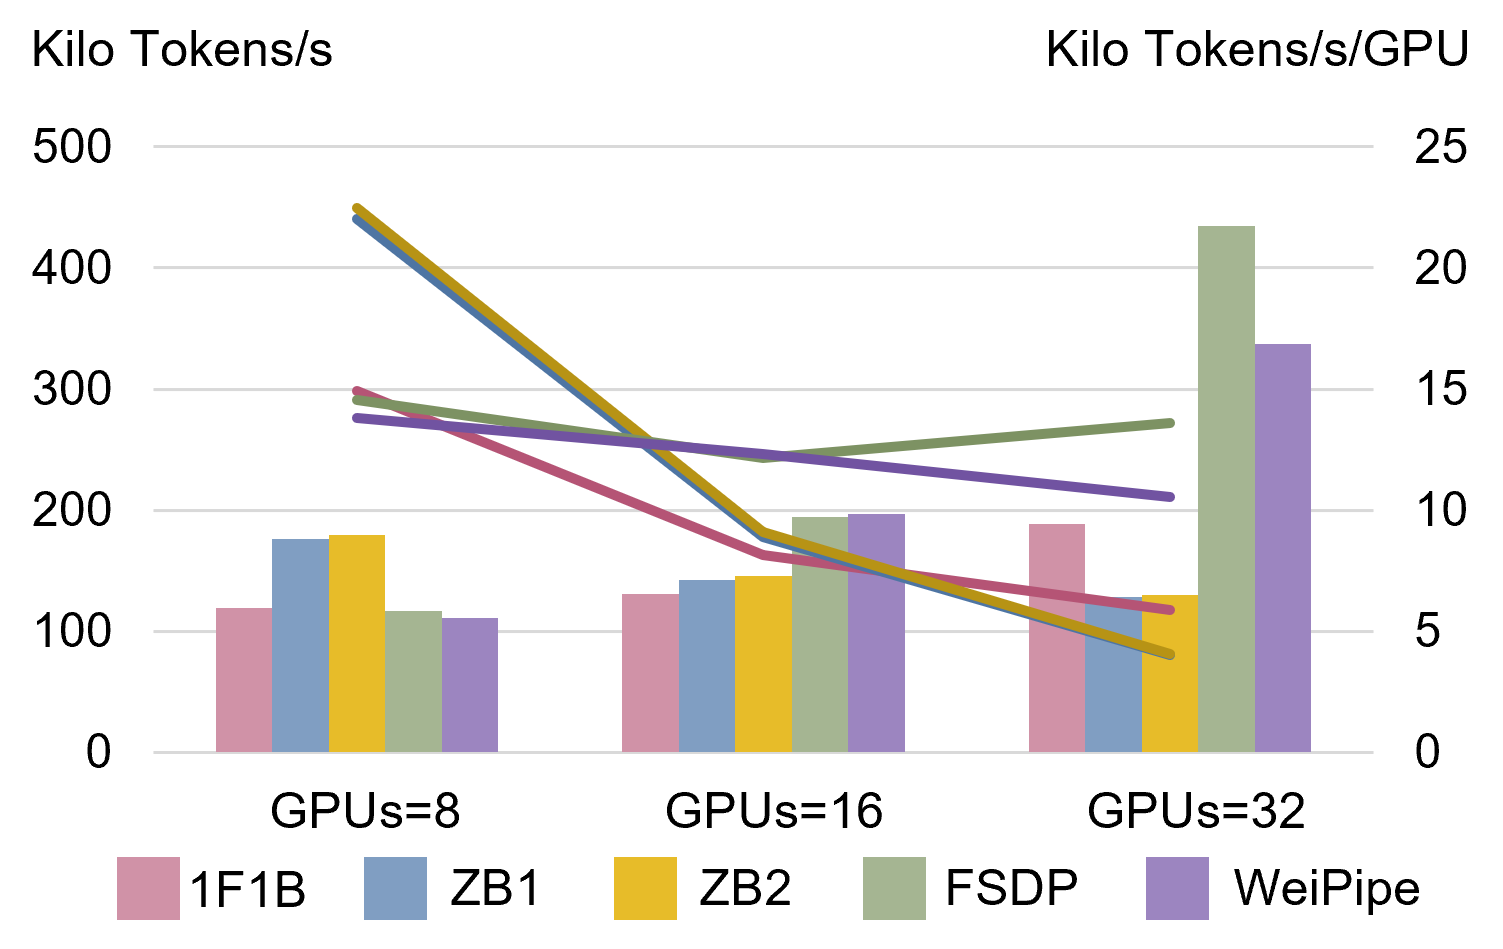
\includegraphics[scale=0.7]{figures/exp_fig3.png}
    \caption{Weak scaling of different strategies. The number of GPUs scales from 8 to 32, and the batch size increases proportionally. The left coordinates correspond to the overall throughput as represented by the bar chart, while the coordinates on the right indicate tokens per second per GPU.}
    \label{fig:weipipe-weak}
\end{figure}

It is unexpected to see lower performance with PCIe connections of WeiPipe-Interleave, especially compared to FSDP. Though profiling, we found the primary inefficiency in WeiPipe-Interleave occurs during the tail of the last backward pass. Worker 0 has to wait for other workers to complete the pipeline while still transferring large blocks of data. This bottleneck is less pronounced with NVLink connections due to their higher bandwidth but becomes more apparent in a PCIe \& IB environment. In contrast, FSDP divides communication into many fine-grained blocks, and high-bandwidth NVLink does not effectively reduce the frequency of interruptions. This result also suggests that further optimization of NCCL in WeiPipe is necessary to achieve ideal performance.

% \begin{figure}[!htb]
%     \centering
%     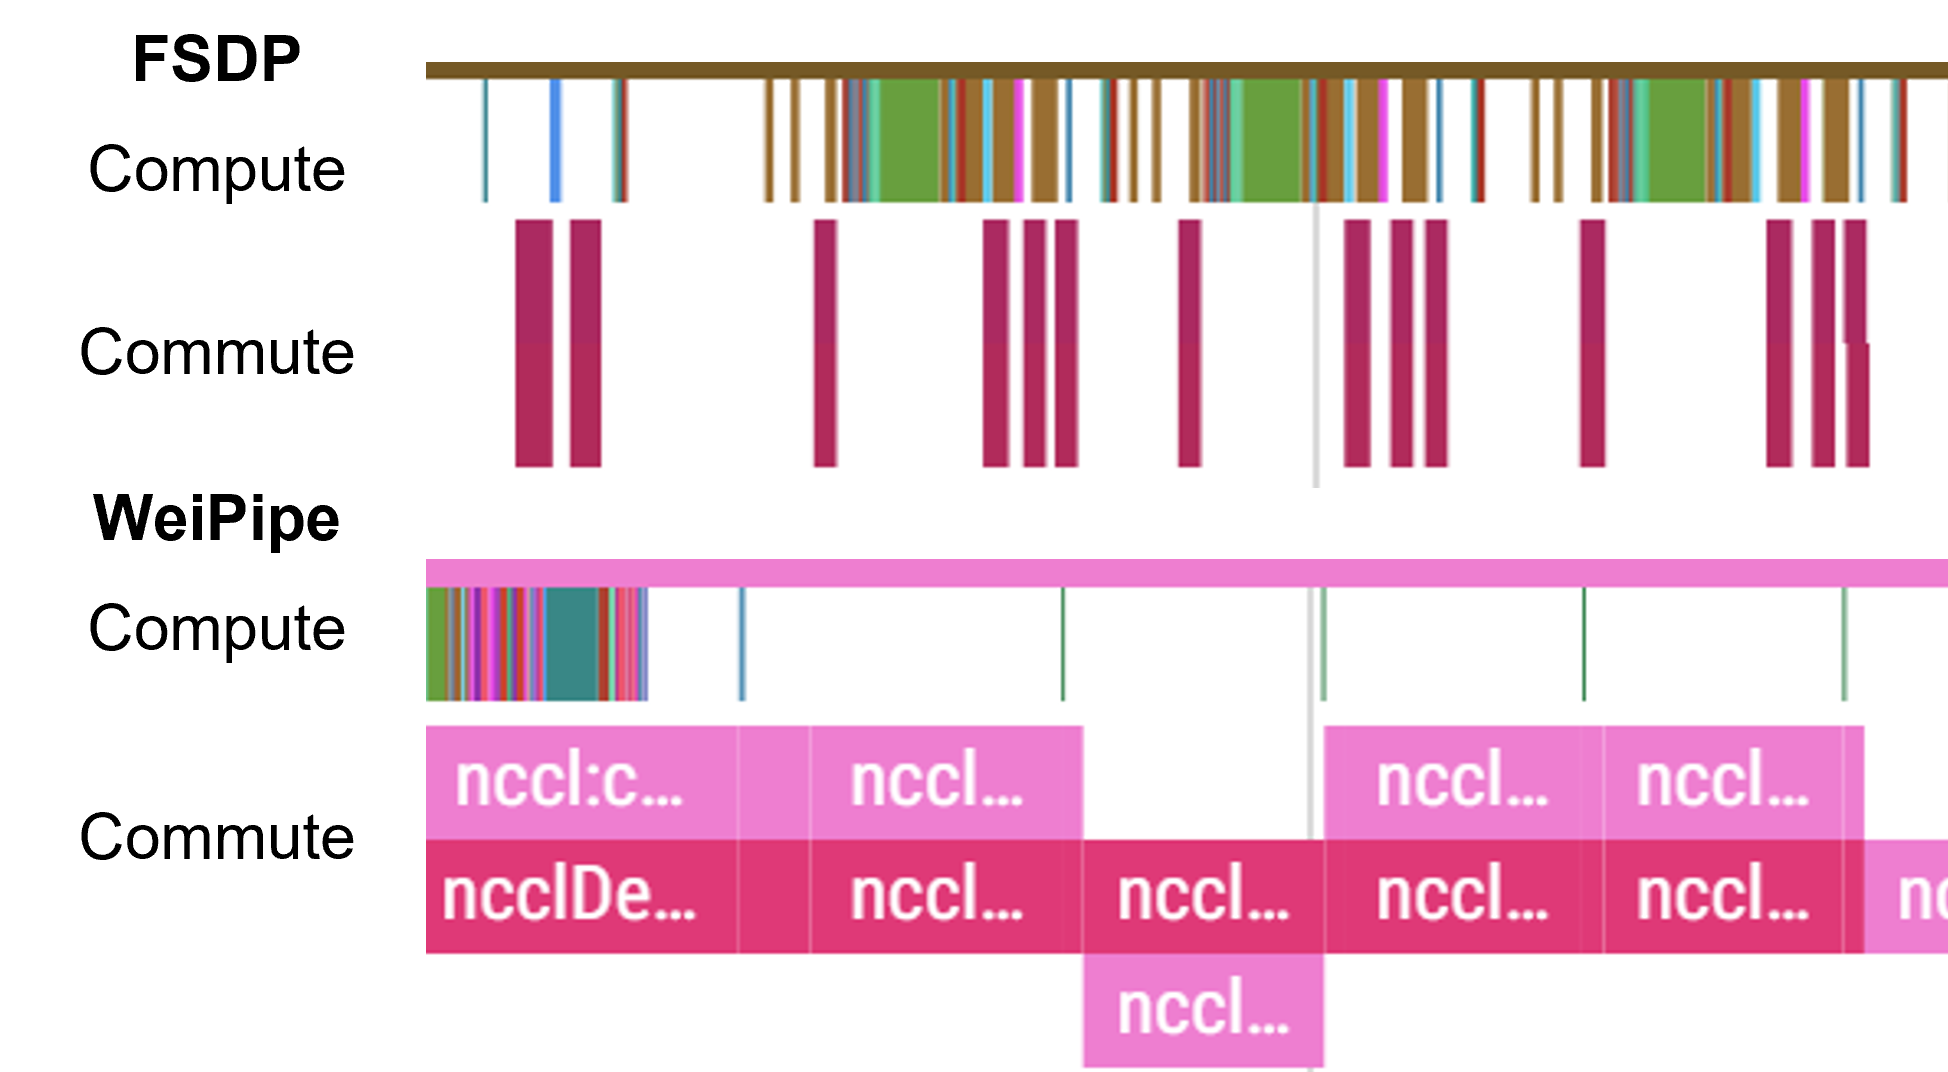
\includegraphics[scale=0.51]{figures/exp_fig1.png}
%     \caption{Bottleneck profiling of FSDP and WeiPipe-Interleave.}
%     \label{fig:weipipe-workload}
% \end{figure}

\subsection{Strong Scaling}

Different from weak scaling, strong scaling measures scalability by keeping the task size constant while expanding the number of workers. In our experiments, the model configuration is the same as the experiments of weak scalability, also increasing the number of GPUs from 8 to 32 
but fix the batch size to 128. The result can be found in Figure \ref{fig:weipipe-strong} and it shows that WeiPipe-Interleave exhibits superior scalability compared to other strategies. This result reveals the WeiPipe-Interleave has the potential to utilize more GPUs to achieve greater speed-up. The large token length and low-bandwidth communication infrastructure cause serious troubles for conventional PP approaches with increasing communication pressure. 

% With more GPUs, the speedup of WeiPipe-Interleave increases from *** to ***. 
% Strong scaling is characterized by maintaining a constant task size while increasing the number of processors. In the context of training a large language model, we attempt to use more GPUs to train the model with a fixed data batch. Here, we use a batch size of 32, which already reaches A100's 80GB memory limit. We then increase the number of GPUs from 8 to 16 and 32, examining whether the total throughput increases proportionally. The results can be found in Figure xxx. 

\begin{figure}[!htb]
    \centering
    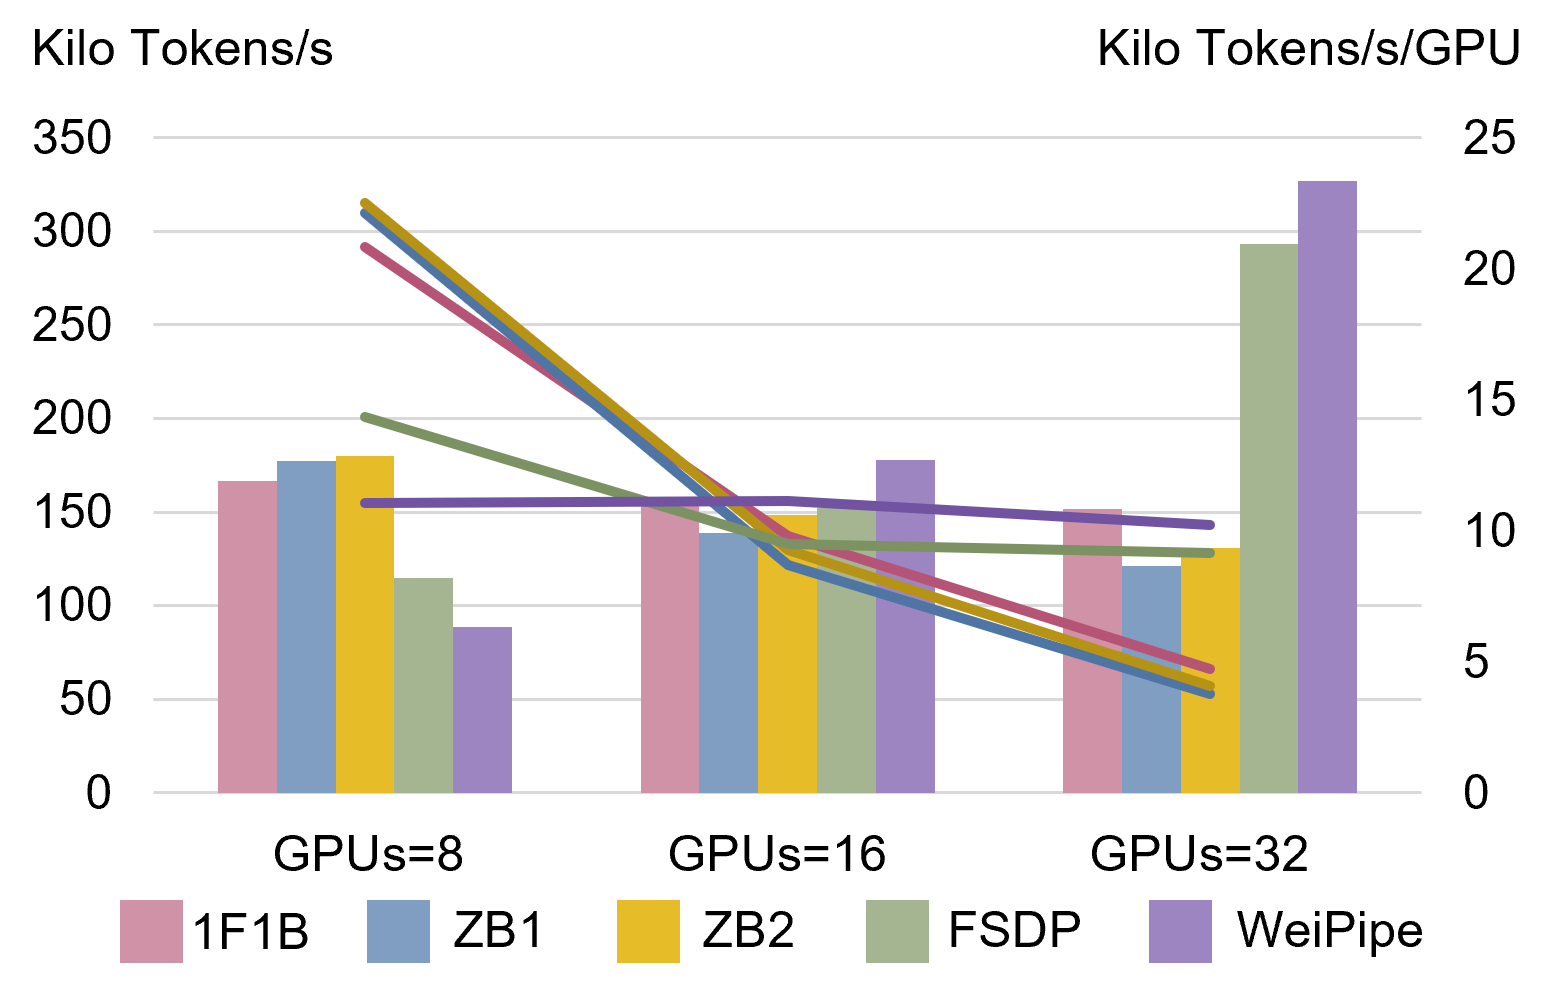
\includegraphics[scale=0.6]{figures/exp_fig4.png}
    \caption{Strong scaling of different strategies. The number of GPUs scales from 8 to 32, but the batch size remains 128.}
    \label{fig:weipipe-strong}
\end{figure}


\section{Conclusions}

In this work, we introduce a novel strategy for pipeline parallelism aimed at reducing communication overhead in LLM training by shifting from activation-based to weight-based communication. We have developed and implemented the WeiPipe-Interleave scheduling technique to minimize the weight-passing overhead, reducing the bubble ratio and balancing memory usage. To further explore the potential of weight-passing pipelines, we discussed the WeiPipe-Zero-Bubble methods to achieve nearly no-vacancy pipelining. Our experiments demonstrate that WeiPipe-Interleave can outperforms current pipeline parallelism approaches and FSDP. WeiPipe extends the prospect of training large-context models with PP and reduces reliance on expensive high-bandwidth communication infrastructure. 

% \section{Acknowlegment}

% Thanks to

% \begin{thebibliography}{00}
% \bibitem{b1} G. Eason, B. Noble, and I. N. Sneddon, ``On certain integrals of Lipschitz-Hankel type involving products of Bessel functions,'' Phil. Trans. Roy. Soc. London, vol. A247, pp. 529--551, April 1955.
% \end{thebibliography}

\bibliographystyle{ACM-Reference-Format}

\bibliography{weipipe}
\end{document}
\endinput
%%
%% End of file `sample-sigplan.tex'.
